\documentclass[10pt]{beamer}

\usetheme{PSY9511}

\usepackage[export]{adjustbox}
\usepackage{hyperref}
\usepackage{listings}
\usepackage{pgfplots}
\usepackage{tikz}
\usepackage{xcolor}

\usepgfplotslibrary{fillbetween}
\usepgfplotslibrary{groupplots}

\usetikzlibrary{arrows}
\usetikzlibrary{arrows.meta}
\usetikzlibrary{calc}
\usetikzlibrary{patterns}
\usetikzlibrary{positioning}

\hypersetup{
    colorlinks=true,
    linkcolor=white,
    urlcolor=blue!80
}

\title{PSY9511: Seminar 8}
\subtitle{Sequence modelling (with an emphasis on language)}
\author{Esten H. Leonardsen}
\date{14.11.24}

\titlegraphic{
	\centering
	\vspace{7.7cm}
	
\includegraphics[width=\logowidth]{data/uio_logo_full.png}
}

\definecolor{firstcolor}{HTML}{ef476f}
\definecolor{secondcolor}{HTML}{ffd166}
\definecolor{thirdcolor}{HTML}{06d6a0}
\definecolor{fourthcolor}{HTML}{118ab2}

\begin{document}
	\begin{frame}
	 	\titlepage
	\end{frame}

    \begin{frame}{Overview}
        \begin{enumerate}
            \item Exercise 5
            \item Language modelling
            \begin{enumerate}
                \item Introduction and motivation
                \item Preprocessing
                \item Bag of words
                \item Vectorization
                \item Recurrent neural networks
                \item Transformers
            \end{enumerate}
        \end{enumerate}
    \end{frame}

    \begin{frame}{Exercise 5}

\begin{enumerate}
    \item Download the Credit.csv dataset from ISL
    \item Preprocess the dataset as you see fit.
    \item Fit one or more non-linear models, choosing model types and hyperparameters according to what you've learned
    \item Report the performance of the best model
    \item Reflect on the choices you made
    \item Reflect upon the performance of the model(s)
\end{enumerate}

\end{frame}


    \section{Language modelling}

    \newcommand{\drawsmiley}[1]{
        \begin{tikzpicture}[scale=0.35]
            % Draw the grid and fill specified cells for the smiley
            \foreach \x in {0,...,9} {
                \foreach \y in {0,...,9} {
                    % Initialize as white
                    \ifnum#1=1
                        \fill[white] (\x,\y) rectangle (\x+1,\y+1);
                    \fi
                    \ifnum#1>1
                        \fill[black!2] (\x,\y) rectangle (\x+1,\y+1);
                    \fi
                }
            }

            \ifnum#1=3
                \foreach \x in {2,...,5} {
                    \foreach \y in {4,...,8} {
                        \fill[white] (\x,\y) rectangle (\x+1,\y+1);
                    }
                }
            \fi

            \fill[black] (3,6) rectangle (4,7);

            \ifnum#1=1
                \fill[black] (6,6) rectangle (7,7);
                \fill[black] (3,4) rectangle (4,5);
                \fill[black] (6,4) rectangle (7,5);
                \fill[black] (4,3) rectangle (6,4);

                % Outline
                \fill[black] (1,2) rectangle (2,8);
                \fill[black] (8,2) rectangle (9,8);
                \fill[black] (2,1) rectangle (8,2);
                \fill[black] (2,8) rectangle (8,9);

                \draw[gray, very thin] (0,0) grid (10,10);
            \fi

            \ifnum#1=3
                \fill[black] (3,4) rectangle (4,5);

                % Outline
                \fill[black] (1,4) rectangle (2,8);
                \fill[black] (2,8) rectangle (6,9);

                \draw[gray, very thin] (1,4) grid (6,9);
            \fi

        \end{tikzpicture}
    }

    \newsavebox{\smiley}
    \sbox{\smiley}{%
        \drawsmiley{1}
    }

    \newsavebox{\eye}
    \sbox{\eye}{%
        \drawsmiley{2}
    }

    \newsavebox{\context}
    \sbox{\context}{%
        \drawsmiley{3}
    }

    \newcommand{\labelnode}[3]{
        \node[text depth=0, text height=0,font=\footnotesize] (#3) at #1 {
            #2
        };
    }

    \newcommand{\embeddingvec}[2]{
        \def\nodesize{12pt}
        \node[draw=black, outer sep=0pt, inner sep=0pt, minimum width=\nodesize, minimum height=\nodesize] (#2n0) at #1 {};
        \node[draw=black, outer sep=0pt, anchor=north, inner sep=0pt, minimum width=\nodesize, minimum height=\nodesize] (#2n1) at (#2n0.south) {};
        \node[draw=black, outer sep=0pt, anchor=north, inner sep=0pt, minimum width=\nodesize, minimum height=\nodesize] (#2n2) at (#2n1.south) {};
        \node[draw=black, outer sep=0pt, anchor=north, inner sep=0pt, minimum width=\nodesize, minimum height=\nodesize] (#2n3) at (#2n2.south) {};
        \node[draw=black, outer sep=0pt, anchor=north, inner sep=0pt, minimum width=\nodesize, minimum height=\nodesize] (#2n4) at (#2n3.south) {};
    }

    \newcommand{\drawsentence}[1]{
        \begin{tikzpicture}
            \def\verticalsep{0.7}
            \node[] at (-1.1, 0.5) {};
            \node[] at (8.4, -5.5) {};

            \node[anchor=west, text depth=0, text height=0] (movie) at (0.65, 0) {
                movie
            };

            \ifnum#1>1
                \node[anchor=west, text depth=0, text height=0] (the) at (0, 0) {
                    The
                };
                \node[anchor=west, text depth=0, text height=0] (was) at (1.67, 0) {
                    was
                };

                \ifnum#1<4
                    \node[anchor=west, text depth=0, text height=0] (great) at (2.33, 0) {
                        great
                    };
                \fi
                \ifnum#1>4
                    \node[anchor=west, text depth=0, text height=0] (great) at (2.33, 0) {
                        great
                    };
                \fi

                \node[anchor=west, text depth=0, text height=0] (comma) at (3.13, 0) {
                    ,
                };
                \node[anchor=west, text depth=0, text height=0] (the2) at (3.25, 0) {
                    the
                };
                \node[anchor=west, text depth=0, text height=0] (actors) at (3.83, 0) {
                    actors
                };
                \node[anchor=west, text depth=0, text height=0] (were) at (4.85, 0) {
                    were
                };

                \ifnum#1<3
                    \node[anchor=west, text depth=0, text height=0] (awesome) at (5.67, 0) {
                        awesome
                    };
                \fi
                \ifnum#1>4
                    \node[anchor=west, text depth=0, text height=0] (awesome) at (5.67, 0) {
                        awesome
                    };
                \fi

                \node[anchor=west, text depth=0, text height=0] (period) at (7.13, 0) {
                    .
                };
            \fi

            \ifnum#1>4
                \ifnum#1<7
                    \node[text depth=0] at (3.6, -6) {\textbf{\textit{Tokenization}}};
                \fi
            \fi

            \ifnum#1=5
                \labelnode{($ (the.south) - (0.15, \verticalsep) $)}{\textcolor{red}{"the"}}{thelabel}
                \labelnode{($ (the.south) - (0.52, \verticalsep) $)}{[}{open}
                \labelnode{($ (period.south) - (-0.45, \verticalsep) $)}{]}{close}
            \fi
            \ifnum#1>5
                \labelnode{($ (the.south) - (0.15, \verticalsep) $)}{"the"}{thelabel}
                \labelnode{($ (the.south) - (1, \verticalsep) $)}{[}{open}
                \labelnode{($ (period.south) - (-1, \verticalsep) $)}{]}{close}
            \fi
            \ifnum#1>4
                \labelnode{($ (movie.south) - (0.15, \verticalsep) $)}{"movie"}{movielabel}
                \labelnode{($ (was.south) - (0.15, \verticalsep) $)}{"was"}{waslabel}
                \labelnode{($ (great.south) - (0.15, \verticalsep) $)}{"great"}{greatlabel}
                \labelnode{($ (comma.south) - (0, \verticalsep) $)}{","}{commalabel}
                \labelnode{($ (the2.south) - (-0.15, \verticalsep) $)}{"the"}{the2label}
                \labelnode{($ (actors.south) - (-0.15, \verticalsep) $)}{"actors"}{actorslabel}
                \labelnode{($ (were.south) - (-0.15, \verticalsep) $)}{"were"}{werelabel}
                \labelnode{($ (awesome.south) - (-0.15, \verticalsep) $)}{"awesome"}{awesomelabel}
                \labelnode{($ (period.south) - (-0.3, \verticalsep) $)}{"."}{periodlabel}

                \draw[-stealth] (the) -- ($ (thelabel.north) + (0, 0.15) $);
                \draw[-stealth] (movie) -- ($ (movielabel.north) + (0, 0.15) $);
                \draw[-stealth] (was) -- ($ (waslabel.north) + (0, 0.15) $);
                \draw[-stealth] (great) -- ($ (greatlabel.north) + (0, 0.15) $);
                \draw[-stealth] (comma) -- ($ (commalabel.north) + (0, 0.15) $);
                \draw[-stealth] (the2) -- ($ (the2label.north) + (0, 0.15) $);
                \draw[-stealth] (actors) -- ($ (actorslabel.north) + (0, 0.15) $);
                \draw[-stealth] (were) -- ($ (werelabel.north) + (0, 0.15) $);
                \draw[-stealth] (awesome) -- ($ (awesomelabel.north) + (0, 0.15) $);
                \draw[-stealth] (period) -- ($ (periodlabel.north) + (0, 0.15) $);

                \ifnum#1=6
                    \labelnode{($ (the.south) - (0.75, \verticalsep) $)}{\textcolor{red}{<s>}}{start}
                    \labelnode{($ (period.south) - (-0.75, \verticalsep) $)}{\textcolor{red}{<e>}}{end}
                \fi

                \ifnum#1>6
                    \labelnode{($ (the.south) - (0.75, \verticalsep) $)}{<s>}{start}
                    \labelnode{($ (period.south) - (-0.75, \verticalsep) $)}{<e>}{end}
                \fi

                \ifnum#1=7
                    \node[text depth=0] at (3.6, -6) {\textbf{\textit{Stemming}}};
                    \labelnode{($ (actorslabel.south) - (0, \verticalsep) $)}{\textcolor{red}{"actor"}}{actorsstem}
                    \labelnode{($ (open.south) - (0, \verticalsep) $)}{[}{openstem}
                    \labelnode{($ (start.south) - (0, \verticalsep) $)}{<s>}{startstem}
                    \labelnode{($ (thelabel.south) - (0, \verticalsep) $)}{"The"}{thestem}
                    \labelnode{($ (movielabel.south) - (0, \verticalsep) $)}{"movie"}{moviestem}
                    \labelnode{($ (waslabel.south) - (0, \verticalsep) $)}{"was"}{wasstem}
                    \labelnode{($ (greatlabel.south) - (0, \verticalsep) $)}{"great"}{greatstem}
                    \labelnode{($ (commalabel.south) - (0, \verticalsep) $)}{","}{commastem}
                    \labelnode{($ (the2label.south) - (-0, \verticalsep) $)}{"the"}{the2stem}
                    \labelnode{($ (werelabel.south) - (0, \verticalsep) $)}{"were"}{werestem}
                    \labelnode{($ (awesomelabel.south) - (0, \verticalsep) $)}{"awesome"}{awesomestem}
                    \labelnode{($ (periodlabel.south) - (0, \verticalsep) $)}{"."}{periodstem}
                    \labelnode{($ (end.south) - (0, \verticalsep) $)}{<e>}{endstem}
                    \labelnode{($ (close.south) - (0, \verticalsep) $)}{]}{closestem}

                    \draw[-stealth] (start) -- ($ (startstem.north) + (0, 0.15) $);
                    \draw[-stealth] (thelabel) -- ($ (thestem.north) + (0, 0.15) $);
                    \draw[-stealth] (movielabel) -- ($ (moviestem.north) + (0, 0.15) $);
                    \draw[-stealth] (waslabel) -- ($ (wasstem.north) + (0, 0.15) $);
                    \draw[-stealth] (greatlabel) -- ($ (greatstem.north) + (0, 0.15) $);
                    \draw[-stealth] (commalabel) -- ($ (commastem.north) + (0, 0.15) $);
                    \draw[-stealth] (the2label) -- ($ (the2stem.north) + (0, 0.15) $);
                    \draw[-stealth] (actorslabel) -- ($ (actorsstem.north) + (0, 0.15) $);
                    \draw[-stealth] (werelabel) -- ($ (werestem.north) + (0, 0.15) $);
                    \draw[-stealth] (awesomelabel) -- ($ (awesomestem.north) + (0, 0.15) $);
                    \draw[-stealth] (periodlabel) -- ($ (periodstem.north) + (0, 0.15) $);
                    \draw[-stealth] (end) -- ($ (endstem.north) + (0, 0.15) $);
                \fi

                \ifnum#1=8
                    \node[text depth=0] at (3.6, -6) {\textbf{\textit{Lemmatization}}};
                    \labelnode{($ (actorslabel.south) - (0, \verticalsep) $)}{\textcolor{red}{"actor"}}{actorsstem}
                    \labelnode{($ (open.south) - (0, \verticalsep) $)}{[}{openstem}
                    \labelnode{($ (start.south) - (0, \verticalsep) $)}{<s>}{startstem}
                    \labelnode{($ (thelabel.south) - (0, \verticalsep) $)}{"The"}{thestem}
                    \labelnode{($ (movielabel.south) - (0, \verticalsep) $)}{"movie"}{moviestem}
                    \labelnode{($ (waslabel.south) - (0, \verticalsep) $)}{"was"}{wasstem}
                    \labelnode{($ (greatlabel.south) - (0, \verticalsep) $)}{"great"}{greatstem}
                    \labelnode{($ (commalabel.south) - (0, \verticalsep) $)}{","}{commastem}
                    \labelnode{($ (the2label.south) - (-0, \verticalsep) $)}{"the"}{the2stem}
                    \labelnode{($ (werelabel.south) - (0, \verticalsep) $)}{\textcolor{red}{"was"}}{werestem}
                    \labelnode{($ (awesomelabel.south) - (0, \verticalsep) $)}{\textcolor{red}{"great"}}{awesomestem}
                    \labelnode{($ (periodlabel.south) - (0, \verticalsep) $)}{"."}{periodstem}
                    \labelnode{($ (end.south) - (0, \verticalsep) $)}{<e>}{endstem}
                    \labelnode{($ (close.south) - (0, \verticalsep) $)}{]}{closestem}

                    \draw[-stealth] (start) -- ($ (startstem.north) + (0, 0.15) $);
                    \draw[-stealth] (thelabel) -- ($ (thestem.north) + (0, 0.15) $);
                    \draw[-stealth] (movielabel) -- ($ (moviestem.north) + (0, 0.15) $);
                    \draw[-stealth] (waslabel) -- ($ (wasstem.north) + (0, 0.15) $);
                    \draw[-stealth] (greatlabel) -- ($ (greatstem.north) + (0, 0.15) $);
                    \draw[-stealth] (commalabel) -- ($ (commastem.north) + (0, 0.15) $);
                    \draw[-stealth] (the2label) -- ($ (the2stem.north) + (0, 0.15) $);
                    \draw[-stealth] (actorslabel) -- ($ (actorsstem.north) + (0, 0.15) $);
                    \draw[-stealth] (werelabel) -- ($ (werestem.north) + (0, 0.15) $);
                    \draw[-stealth] (awesomelabel) -- ($ (awesomestem.north) + (0, 0.15) $);
                    \draw[-stealth] (periodlabel) -- ($ (periodstem.north) + (0, 0.15) $);
                    \draw[-stealth] (end) -- ($ (endstem.north) + (0, 0.15) $);
                \fi

                \ifnum#1=9
                    \node[text depth=0] at (3.6, -6) {\textbf{\textit{Stopword removal}}};
                    \labelnode{($ (open.south) - (0, \verticalsep) $)}{[}{openstem}
                    \labelnode{($ (start.south) - (0, \verticalsep) $)}{<s>}{startstem}
                    \labelnode{($ (movielabel.south) - (0, \verticalsep) $)}{"movie"}{moviestem}
                    \labelnode{($ (greatlabel.south) - (0, \verticalsep) $)}{"great"}{greatstem}
                    \labelnode{($ (commalabel.south) - (0, \verticalsep) $)}{","}{commastem}
                    \labelnode{($ (actorslabel.south) - (0, \verticalsep) $)}{"actor"}{actorsstem}
                    \labelnode{($ (awesomelabel.south) - (0, \verticalsep) $)}{"awesome"}{awesomestem}
                    \labelnode{($ (periodlabel.south) - (0, \verticalsep) $)}{"."}{periodstem}
                    \labelnode{($ (end.south) - (0, \verticalsep) $)}{<e>}{endstem}
                    \labelnode{($ (close.south) - (0, \verticalsep) $)}{]}{closestem}

                    \draw[-stealth] (start) -- ($ (startstem.north) + (0, 0.15) $);
                    \draw[-stealth] (movielabel) -- ($ (moviestem.north) + (0, 0.15) $);
                    \draw[-stealth] (greatlabel) -- ($ (greatstem.north) + (0, 0.15) $);
                    \draw[-stealth] (commalabel) -- ($ (commastem.north) + (0, 0.15) $);
                    \draw[-stealth] (actorslabel) -- ($ (actorsstem.north) + (0, 0.15) $);
                    \draw[-stealth] (awesomelabel) -- ($ (awesomestem.north) + (0, 0.15) $);
                    \draw[-stealth] (periodlabel) -- ($ (periodstem.north) + (0, 0.15) $);
                    \draw[-stealth] (end) -- ($ (endstem.north) + (0, 0.15) $);
                \fi

                \ifnum#1>9
                    \ifnum#1<12
                        \node[font=\small] (dictionary) at (3.8, -3) {
                            ["," "." <e> <s> "actors" "awesome" "great" "movie" "the" "was" "were"]
                        };

                        \node[anchor=north, font=\footnotesize] at ($ (dictionary.south) - (4.55, -0.2) $) {
                            \textcolor{red}{0}
                        };
                        \node[anchor=north, font=\footnotesize] at ($ (dictionary.south) - (4.23, -0.2) $) {
                            \textcolor{red}{1}
                        };
                        \node[anchor=north, font=\footnotesize] at ($ (dictionary.south) - (3.77, -0.2) $) {
                            \textcolor{red}{2}
                        };
                        \node[anchor=north, font=\footnotesize] at ($ (dictionary.south) - (3.2, -0.2) $) {
                            \textcolor{red}{3}
                        };
                        \node[anchor=north, font=\footnotesize] at ($ (dictionary.south) - (2.3, -0.2) $) {
                            \textcolor{red}{4}
                        };
                        \node[anchor=north, font=\footnotesize] at ($ (dictionary.south) - (0.9, -0.2) $) {
                            \textcolor{red}{5}
                        };
                        \node[anchor=north, font=\footnotesize] at ($ (dictionary.south) - (-0.4, -0.2) $) {
                            \textcolor{red}{6}
                        };
                        \node[anchor=north, font=\footnotesize] at ($ (dictionary.south) - (-1.5, -0.2) $) {
                            \textcolor{red}{7}
                        };
                        \node[anchor=north, font=\footnotesize] at ($ (dictionary.south) - (-2.45, -0.2) $) {
                            \textcolor{red}{8}
                        };
                        \node[anchor=north, font=\footnotesize] at ($ (dictionary.south) - (-3.35, -0.2) $) {
                            \textcolor{red}{9}
                        };
                        \node[anchor=north, font=\footnotesize] at ($ (dictionary.south) - (-4.2, -0.2) $) {
                            \textcolor{red}{10}
                        };
                    \fi
                    \ifnum#1>10
                        \ifnum#1<13
                            \node[text depth=0] at (3.6, -6) {\textbf{\textit{Integer encoding}}};
                        \fi
                        \labelnode{($ (open.south) - (0, \verticalsep) $)}{[}{open}
                        \labelnode{($ (start.south) - (0, \verticalsep) $)}{3}{startstem}
                        \labelnode{($ (thelabel.south) - (0, \verticalsep) $)}{8}{thestem}
                        \labelnode{($ (movielabel.south) - (0, \verticalsep) $)}{7}{moviestem}
                        \labelnode{($ (waslabel.south) - (0, \verticalsep) $)}{9}{wasstem}
                        \labelnode{($ (greatlabel.south) - (0, \verticalsep) $)}{6}{greatstem}
                        \labelnode{($ (commalabel.south) - (0, \verticalsep) $)}{0}{commastem}
                        \labelnode{($ (the2label.south) - (-0, \verticalsep) $)}{8}{the2stem}
                        \labelnode{($ (actorslabel.south) - (0, \verticalsep) $)}{4}{actorsstem}
                        \labelnode{($ (werelabel.south) - (0, \verticalsep) $)}{10}{werestem}
                        \labelnode{($ (awesomelabel.south) - (0, \verticalsep) $)}{5}{awesomestem}
                        \labelnode{($ (periodlabel.south) - (0, \verticalsep) $)}{1}{periodstem}
                        \labelnode{($ (end.south) - (0, \verticalsep) $)}{2}{endstem}
                        \labelnode{($ (close.south) - (0, \verticalsep) $)}{]}{closestem}

                        \draw[-stealth] (start) -- ($ (startstem.north) + (0, 0.15) $);
                        \draw[-stealth] (thelabel) -- ($ (thestem.north) + (0, 0.15) $);
                        \draw[-stealth] (movielabel) -- ($ (moviestem.north) + (0, 0.15) $);
                        \draw[-stealth] (waslabel) -- ($ (wasstem.north) + (0, 0.15) $);
                        \draw[-stealth] (greatlabel) -- ($ (greatstem.north) + (0, 0.15) $);
                        \draw[-stealth] (commalabel) -- ($ (commastem.north) + (0, 0.15) $);
                        \draw[-stealth] (the2label) -- ($ (the2stem.north) + (0, 0.15) $);
                        \draw[-stealth] (actorslabel) -- ($ (actorsstem.north) + (0, 0.15) $);
                        \draw[-stealth] (werelabel) -- ($ (werestem.north) + (0, 0.15) $);
                        \draw[-stealth] (awesomelabel) -- ($ (awesomestem.north) + (0, 0.15) $);
                        \draw[-stealth] (periodlabel) -- ($ (periodstem.north) + (0, 0.15) $);
                        \draw[-stealth] (end) -- ($ (endstem.north) + (0, 0.15) $);
                    \fi
                \fi
            \fi
            \ifnum#1>13
                \embeddingvec{($ (moviestem.south) - (0, \verticalsep) $)}{movie}
                \embeddingvec{($ (greatstem.south) - (0, \verticalsep) $)}{great}
                \embeddingvec{($ (actorsstem.south) - (0, \verticalsep) $)}{actors}
                \embeddingvec{($ (awesomestem.south) - (0, \verticalsep) $)}{awesome}
                \draw[-stealth] (moviestem) -- (movien0);
                \draw[-stealth] (greatstem) -- (greatn0);
                \draw[-stealth] (actorsstem) -- (actorsn0);
                \draw[-stealth] (awesomestem) -- (awesomen0);

                \ifnum#1<15
                    \embeddingvec{($ (startstem.south) - (0, \verticalsep) $)}{start}
                    \embeddingvec{($ (thestem.south) - (0, \verticalsep) $)}{the}
                    \embeddingvec{($ (wasstem.south) - (0, \verticalsep) $)}{was}
                    \embeddingvec{($ (commastem.south) - (0, \verticalsep) $)}{comma}
                    \embeddingvec{($ (the2stem.south) - (0, \verticalsep) $)}{the2}
                    \embeddingvec{($ (werestem.south) - (0, \verticalsep) $)}{were}
                    \embeddingvec{($ (periodstem.south) - (0, \verticalsep) $)}{period}
                    \embeddingvec{($ (endstem.south) - (0, \verticalsep) $)}{end}
                    \draw[-stealth] (thestem) -- (then0);
                    \draw[-stealth] (wasstem) -- (wasn0);
                    \draw[-stealth] (commastem) -- (comman0);
                    \draw[-stealth] (the2stem) -- (the2n0);
                    \draw[-stealth] (werestem) -- (weren0);
                    \draw[-stealth] (periodstem) -- (periodn0);
                    \draw[-stealth] (startstem) -- (startn0);
                    \draw[-stealth] (endstem) -- (endn0);
                \fi
            \fi
            \ifnum#1>15

            \fi

        \end{tikzpicture}
    }

    \newsavebox{\onlymovie}
    \sbox{\onlymovie}{%
        \drawsentence{1}
    }
    \newsavebox{\sentence}
    \sbox{\sentence}{%
        \drawsentence{2}
    }
    \newsavebox{\sentencewithgaps}
    \sbox{\sentencewithgaps}{%
        \drawsentence{3}
    }
    \newsavebox{\sentencewithmanygaps}
    \sbox{\sentencewithmanygaps}{%
        \drawsentence{4}
    }
    \newsavebox{\tokenizedsentence}
    \sbox{\tokenizedsentence}{%
        \drawsentence{5}
    }
    \newsavebox{\startendsentence}
    \sbox{\startendsentence}{%
        \drawsentence{6}
    }
    \newsavebox{\stemmedsentence}
    \sbox{\stemmedsentence}{%
        \drawsentence{7}
    }
    \newsavebox{\lemmatizedsentence}
    \sbox{\lemmatizedsentence}{%
        \drawsentence{8}
    }
    \newsavebox{\prunedsentence}
    \sbox{\prunedsentence}{%
        \drawsentence{9}
    }
    \newsavebox{\sentencedictionary}
    \sbox{\sentencedictionary}{%
        \drawsentence{10}
    }
    \newsavebox{\encodingsentence}
    \sbox{\encodingsentence}{%
        \drawsentence{11}
    }
    \newsavebox{\encodedsentence}
    \sbox{\encodedsentence}{%
        \drawsentence{12}
    }
    \newsavebox{\encodedsentencenolabel}
    \sbox{\encodedsentencenolabel}{%
        \drawsentence{13}
    }
    \newsavebox{\embeddedsentence}
    \sbox{\embeddedsentence}{%
        \drawsentence{14}
    }
    \newsavebox{\positionalsentence}
    \sbox{\positionalsentence}{%
        \drawsentence{15}
    }
    \newsavebox{\countpositional}
    \sbox{\countpositional}{%
        \drawsentence{16}
    }
    \newsavebox{\normalizedpositional}
    \sbox{\normalizedpositional}{%
        \drawsentence{17}
    }

    \begin{frame}{Introduction}
        \only<1-29>{
            \begin{tikzpicture}
                \node[] at (0, 0) {};
                \node[] at (10, 7) {};

                \only<2-4,7-8>{
                    \node[] at (3, 2) {
                        {\footnotesize
                            \begin{tabular}{|c|c|c|c|}
                                \hline
                                Age&Sex&Education&Salary \\ \hline
                                25 & Male & 12 & 40,000 \\ \hline
                                30 & Female & 16 & 65,000 \\ \hline
                                35 & Male & 14 & 55,000 \\ \hline
                                40 & Female & 18 & 80,000 \\ \hline
                                45 & Male & 16 & 75,000 \\ \hline
                            \end{tabular}
                        }
                    };
                }
                \only<3-4,7,11,14>{
                    \node[] at (8, 2) {
                        \usebox{\smiley}
                    };
                }
                \only<4-7,15,17-21,26-27>{
                    \node[anchor=north, inner sep=0pt, outer sep=0pt] at (5.3, 6.7) {
                        \usebox{\sentence}
                    };
                }
                \only<5-6>{
                    \node[inner sep=0pt, draw=black] at (5.5, 4) {
                        
\includegraphics[width=5cm]{data/soundwaves.png}
                    };
                }
                \only<6>{
                    \node[inner sep=0pt, draw=black] at (5.5, 1.5) {
                        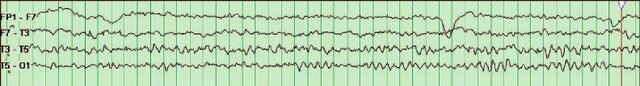
\includegraphics[width=8cm]{data/eeg.jpeg}
                    };
                }
                \only<9-10>{
                    \node[] at (0.84, 2.98) {
                        \footnotesize{Age}
                    };
                    \node[] at (0.84, 1.82) {
                        \footnotesize{35}
                    };
                }
                \only<10>{
                    \node[] at (1.93, 3.02) {
                        \footnotesize{Sex}
                    };
                    \node[] at (1.93, 1.83) {
                        \footnotesize{Male}
                    };

                }
                \only<12>{
                    \node[] at (8, 2) {
                        \usebox{\eye}
                    };
                }
                \only<13>{
                    \node[] at (8, 2) {
                        \usebox{\context}
                    };
                }
                \only<16>{
                    \node[anchor=north, inner sep=0pt, outer sep=0pt] at (5.3, 6.7) {
                        \usebox{\onlymovie}
                    };
                }
                \only<18-19>{
                    \node[] (pos) at (5, 4) {
                        \textcolor{green}{Positive}
                    };
                    \node[] (neg) at (5, 3) {
                        \textcolor{red}{Negative}
                    };
                };
                \only<19>{
                    \node[] at (5, 0.9) {
                        The movie was awful, the actors were horrible.
                    };
                    \node[minimum width=0.95cm, minimum height=0.35cm, draw=red, thick] (awful) at (4.2, 0.92) {};
                    \node[minimum width=1.35cm, minimum height=0.35cm, draw=red, thick] (horrible) at (7.95, 0.92) {};
                    \node[minimum width=0.88cm, minimum height=0.35cm, draw=green, thick] (great) at (4.47, 6.15) {};
                    \node[minimum width=1.56cm, minimum height=0.35cm, draw=green, thick] (awesome) at (8.15, 6.15) {};

                    \draw[green, -stealth] (great) -- (pos);
                    \draw[green, -stealth] (awesome) -- (pos);
                    \draw[red, -stealth] (awful) -- (neg);
                    \draw[red, -stealth] (horrible) -- (neg);
                }
                \only<20-21>{
                    \node[] at (5.25, 4) {
                        La película fue genial, las actores fueron increíbles.
                    };
                }
                \only<21>{
                    \draw[-stealth] (2, 5.9) -- (1.5, 4.2);
                    \draw[-stealth] (2.85, 5.9) -- (2.35, 4.2);
                    \draw[-stealth] (3.75, 5.9) -- (3.25, 4.2);
                    \draw[-stealth] (4.55, 5.9) -- (4.05, 4.2);
                    \draw[-stealth] (5.21, 5.9) -- (4.95, 4.2);
                    \draw[-stealth] (6.05, 5.9) -- (5.9, 4.2);
                    \draw[-stealth] (7, 5.9) -- (7.05, 4.2);
                    \draw[-stealth] (8.2, 5.9) -- (8.45, 4.2);
                }
                \only<22,25>{
                    \node[anchor=north, inner sep=0pt, outer sep=0pt] at (5.3, 6.7) {
                        \usebox{\sentencewithgaps}
                    };
                }
                \only<22,24-25>{
                    \draw[thick] (7.3, 6) -- (8.8, 6);
                }
                \only<23>{
                    \draw[thick] (1.5, 6) -- (8.8, 6);
                }
                \only<24>{
                    \node[anchor=north, inner sep=0pt, outer sep=0pt] at (5.3, 6.7) {
                        \usebox{\sentencewithmanygaps}
                    };
                    \draw[thick] (4.1, 6) -- (4.9, 6);
                }
                \only<27>{
                    \node[minimum width=0.88cm, minimum height=0.35cm, draw=black, thick] (great) at (4.47, 6.15) {};
                    \node[minimum width=1.56cm, minimum height=0.35cm, draw=black, thick] (awesome) at (8.15, 6.15) {};
                    \draw[-stealth] (great) to [out=315, in=225] (awesome);
                }
                \only<28>{
                    \node[align=center, anchor=north] at (5.0, 6.45) {
                        The movie was great, we saw it at the new\\Cinema in the city center, the actors were awesome.
                    };
                    \node[minimum width=0.88cm, minimum height=0.35cm, draw=black, thick] (great) at (4.55, 6.15) {};
                    \node[minimum width=1.56cm, minimum height=0.35cm, draw=black, thick] (awesome) at (8.25, 5.7) {};
                }
                \only<29>{
                    \node[align=center, anchor=north] at (5.0, 6.45) {
                        The movie was great, we saw it at the new\\
                        Cinema in the city center, right down by the\\
                        restaurant where we went for my birthday that\\
                        one year, the one where the clown was\\
                        inside the cake, the actors were awesome.
                    };
                    \node[minimum width=0.88cm, minimum height=0.35cm, draw=black, thick] (great) at (4.55, 6.15) {};
                    \node[minimum width=1.56cm, minimum height=0.35cm, draw=black, thick] (awesome) at (7.5, 4.25) {};
                }

            \end{tikzpicture}
        }
        \only<30>{
            Language modelling: Using the innate structure in language to create better models
            \begin{itemize}
                \item Classification: Predict a class for a full sequence (sentiment analysis)
                \item Sequence-to-sequence: Predict a sequence from another sequence (translation)
                \item Generative: Predict the next token in a sequence of words
            \end{itemize}
        }
    \end{frame}

    \section{Preprocessing}

    \begin{frame}[fragile,t]{Preprocessing}
        \only<1-13>{
            \begin{tikzpicture}
                \centering
                \node[] at (0, 0) {};
                \node[] at (10, 7) {};

                \only<1>{
                    \node[anchor=north] at (5, 7.2) {
                        \usebox{\sentence}
                    };
                }
                \only<2>{
                    \node[anchor=north] at (5, 7.2) {
                        \usebox{\tokenizedsentence}
                    };
                }
                \only<3-4>{
                    \node[anchor=north] at (5, 7.2) {
                        \usebox{\startendsentence}
                    };
                }
                \only<4>{
                    \PythonInputNode{1}{(1.05, 4.9)}{import}{0.9\textwidth}{7}{
    from nltk.tokenize import word_tokenize^^J
    ^^J
    tokens = word_tokenize(s)^^J
    tokens = [token.lower() for token in tokens]^^J
    tokens = ['<s>'] + tokens + ['<e>']^^J
    print(tokens)^^J
                    }
                    \PythonOutputNode{1}{(1.16, 3)}{out}{0.79\textwidth}{7}{
                        ['<s>', 'the', 'movie', 'was', 'great', ',', 'the', 'actors',^^J
                        'were', 'awesome', '.', '<e>']^^J
                    }
                }
                \only<5-6>{
                    \node[anchor=north] at (5, 7.2) {
                        \usebox{\stemmedsentence}
                    };
                }
                \only<6>{

                    \PythonInputNode{1}{(1.05, 4.3)}{import}{0.9\textwidth}{7}{
    from nltk.stem.snowball import SnowballStemmer^^J
    ^^J
    stemmer = SnowballStemmer('english')^^J
    stemmed = [stemmer.stem(token) for token in tokens]^^J
    stemmed^^J
                    }
                    \PythonOutputNode{1}{(1.16, 2.7)}{out}{0.79\textwidth}{7}{
    ['<s>', 'the', 'movi', 'was', 'great', ',', 'the', 'actor', ^^J
    'were', 'awesom', '.', '<e>']^^J
                    }
                }
                \only<7-8>{
                    \node[anchor=north] at (5, 7.2) {
                        \usebox{\lemmatizedsentence}
                    };
                }
                \only<8>{
                    \PythonInputNode{1}{(1.05, 4.3)}{import}{0.9\textwidth}{7}{
    from nltk.stem import WordNetLemmatizer^^J
    ^^J
    lemmatizer = WordNetLemmatizer()^^J
    lemmatized = [lemmatizer.lemmatize(token) for token in tokens]^^J
    print(lemmatized)^^J
                    }
                    \PythonOutputNode{1}{(1.16, 2.7)}{out}{0.79\textwidth}{7}{
    ['<s>', 'the', 'movie', 'wa', 'great', ',', 'the', 'actor',^^J
    'were', 'awesome', '.', '<e>']^^J
                    }
                }
                \only<9-10>{
                    \node[anchor=north] at (5, 7.2) {
                        \usebox{\prunedsentence}
                    };
                }
                \only<10>{
                    \PythonInputNode{1}{(1.05, 4.3)}{import}{0.9\textwidth}{7}{
    from nltk.corpus import stopwords^^J
    ^^J
    pruned = [token for token in tokens if not token in stopwords.words('english')]^^J
    print(pruned)^^J
                    }
                    \PythonOutputNode{1}{(1.16, 2.7)}{out}{0.79\textwidth}{7}{
    ['<s>', 'movie', 'great', ',', 'actors', 'awesome', '.', '<e>']^^J
                    }
                }
                \only<11>{
                    \node[anchor=north] at (5, 7.2) {
                        \usebox{\sentencedictionary}
                    };
                }
                \only<12>{
                    \node[anchor=north] at (5, 7.2) {
                        \usebox{\encodingsentence}
                    };
                }
                \only<13>{
                    \node[anchor=north] at (5, 7.2) {
                        \usebox{\encodedsentence}
                    };
                }
            \end{tikzpicture}
        }
        \only<14>{
            Language preprocessing: Highlighting important parts of a sentence while hiding redundancies
            \begin{itemize}
                \item Tokenization: Splitting text into tokens
                \item Stemming: Removing redundant suffixes
                \item Lemmatization: Mapping words to common lemmas
                \item Stopword removal: Removing non-informative words
                \item Integer encoding: Turning words into numbers
                \item \textbf{Assumes we know what is important and what is redundant}
            \end{itemize}
        }
    \end{frame}

    \newsavebox{\wordcounts}
    \sbox{\wordcounts}{%
        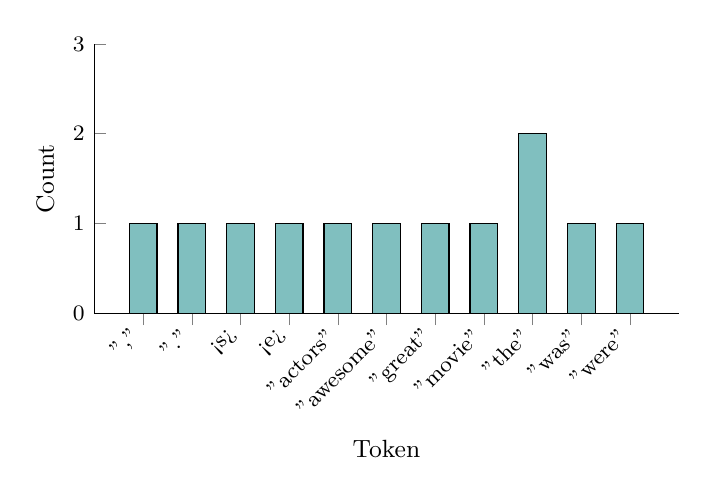
\begin{tikzpicture}
            \begin{axis}[
                ybar,
                ymin=0,
                ymax=3,
                height=5cm,
                width=9cm,
                xtick={0, 1, 2, 3, 4, 5, 6, 7, 8, 9, 10},
                xticklabels={{","}, {"."}, <s>, <e>, "actors", "awesome", "great", "movie", "the", "was", "were"},
                xticklabel style={font=\footnotesize, rotate=45, anchor=east},
                yticklabel style={font=\footnotesize},
                xlabel={\small{Token}},
                ylabel={\small{Count}},
                axis y line*=left,
                axis x line*=bottom
            ]
                \addplot[fill=teal!50] coordinates {
                    (0, 1)
                    (1, 1)
                    (2, 1)
                    (3, 1)
                    (4, 1)
                    (5, 1)
                    (6, 1)
                    (7, 1)
                    (8, 2)
                    (9, 1)
                    (10, 1)
                };
            \end{axis}
        \end{tikzpicture}
    }

    \section{Bag of words}
    \begin{frame}[t]{Bag of words}
        \begin{tikzpicture}
            \node[] at (0, 0) {};
            \node[] at (10, 7) {};

            \only<1-5>{
                \node[anchor=north] at (5, 7) {
                    \usebox{\sentence}
                };
            }

            \only<2>{
                \node[] at (5, 2.8) {
                    \usebox{\wordcounts}
                };
            }

            \only<3>{
                \node[anchor=north west] at (0.2, 5.8) {
                    {
                        \scriptsize
                        \setlength{\tabcolsep}{1.5pt}
                        \begin{tabular}{|c|c|c|c|c|c|c|c|c|c|c|}
                            \hline
                            ,&.&<s>&<e>&actors&awesome&great&movie&the&was&were\\
                            \hline
                            1&1&1&1&1&1&1&1&2&1&1\\
                            \hline
                        \end{tabular}
                    }
                };
            }
            \only<4,6>{
                \node[anchor=north west] at (0.2, 5.8) {
                    {
                        \scriptsize
                        \setlength{\tabcolsep}{1.5pt}
                        \begin{tabular}{|c|c|c|c|c|c|c|c|c|c|c|c|c|c|}
                            \hline
                            ,&.&<s>&<e>&actors&awesome&awful&great&horrible&movie&the&was&were&sentiment\\
                            \hline
                            1&1&1&1&1&1&0&1&0&1&2&1&1&positive\\
                            \hline
                            1&1&1&1&1&0&1&0&1&1&2&1&1&negative\\
                            \hline
                        \end{tabular}
                    }
                };
            }
            \only<4-5>{
                \node[] at (5, 4) {
                    The movie was awful, the actors were horrible.
                };
            }
            \only<5>{
                \node[anchor=north west] at (0.2, 5.8) {
                    {
                        \scriptsize
                        \setlength{\tabcolsep}{1.5pt}
                        \begin{tabular}{|c|c|c|c|c|c|c|c|c|c|c|c|c|c|}
                            \hline
                            ,&.&<s>&<e>&actors&\textcolor{red}{awesome}&\textcolor{red}{awful}&\textcolor{red}{great}&\textcolor{red}{horrible}&movie&the&was&were&sentiment\\
                            \hline
                            1&1&1&1&1&\textcolor{red}{1}&\textcolor{red}{0}&\textcolor{red}{1}&\textcolor{red}{0}&1&2&1&1&positive\\
                            \hline
                            1&1&1&1&1&\textcolor{red}{0}&\textcolor{red}{1}&\textcolor{red}{0}&\textcolor{red}{1}&1&2&1&1&negative\\
                            \hline
                        \end{tabular}
                    }
                };
            }
            \only<6>{
                \node[] at (5, 3.3) {
                    $y=\beta_0 + \sum\limits_i \beta_iX_i$
                };
            }

            \only<7>{
                \node[] at (5, 3.3) {
                    {\scriptsize
                        \url{http://localhost:8888/notebooks/notebooks/Bag\%20of\%20words.ipynb}
                    }
                };
            }

        \end{tikzpicture}
    \end{frame}

    \begin{frame}{Bag of words}
        Bag of words: Model language by using word counts (or frequencies)
        \begin{itemize}
            \item Main advantage: Simple, useful when a few key words are sufficient to determine the correct prediction
            \item Main disadvantage: Does not understand word similarities
        \end{itemize}
    \end{frame}

    \newcommand{\pointcloud}[1]{
        \begin{tikzpicture}
            \begin{axis}[
                xmin=0.35,
                xmax=0.7,
                ymin=0.35,
                ymax=0.7,
                height=6cm,
                width=6cm,
                xmajorticks=false,
                ymajorticks=false
            ]

            \ifnum#1=1
                \addplot[
                    only marks,
                    mark=*,
                    color=gray!80,
                    opacity=0.75
                ] coordinates {
                    (0.5, 0.5)
                    (0.52, 0.53)
                    (0.48, 0.55)
                    (0.45, 0.47)
                    (0.57, 0.46)
                    (0.53, 0.51)
                    (0.47, 0.52)
                    (0.49, 0.50)
                    (0.51, 0.54)
                    (0.5, 0.56)
                    (0.55, 0.55)
                    (0.58, 0.57)
                    (0.54, 0.59)
                    (0.52, 0.53)
                    (0.57, 0.56)
                    (0.59, 0.54)
                    (0.56, 0.58)
                    (0.60, 0.55)
                    (0.53, 0.52)
                    (0.56, 0.53)
                };
            \fi

            \ifnum#1>1
                \addplot[
                    only marks,
                    mark=*,
                    color=blue!80,
                    opacity=0.75
                ] coordinates {
                    (0.5, 0.5)
                    (0.52, 0.53)
                    (0.48, 0.55)
                    (0.45, 0.47)
                    (0.57, 0.46)
                    (0.53, 0.51)
                    (0.47, 0.52)
                    (0.49, 0.50)
                    (0.51, 0.54)
                    (0.5, 0.56)
                };

                \addplot[
                    only marks,
                    mark=*,
                    color=red!80,
                    opacity=0.75
                ] coordinates {
                    (0.55, 0.55)
                    (0.58, 0.57)
                    (0.54, 0.59)
                    (0.52, 0.53)
                    (0.57, 0.56)
                    (0.59, 0.54)
                    (0.56, 0.58)
                    (0.60, 0.55)
                    (0.53, 0.52)
                    (0.56, 0.53)
                };
            \fi
            \ifnum#1=3
                \addplot[dashed] coordinates {
                    (0.15,0.9)
                    (0.75, 0.3)
                };
            \fi
            \end{axis}
        \end{tikzpicture}
    }

    \newsavebox{\singlecloud}
    \sbox{\singlecloud}{%
        \pointcloud{1}
    }
    \newsavebox{\doublecloud}
    \sbox{\doublecloud}{%
        \pointcloud{2}
    }
    \newsavebox{\boundarycloud}
    \sbox{\boundarycloud}{%
        \pointcloud{3}
    }

    \newsavebox{\oppositevectors}
    \sbox{\oppositevectors}{%
        \begin{tikzpicture}
            \begin{axis}[
                axis lines=middle,
                xmin=-1.2,
                xmax=1.2,
                ymin=-1.2,
                ymax=1.2,
                axis line style={
                    draw=gray!50,
                    stealth-stealth
                },
                tick label style={
                    font=\small,
                    gray!50
                },
                clip=false
            ]
                \node[circle, fill=blue, label=above:\footnotesize{awesome}, opacity=0.5] at (axis cs: 1, 0) {};
                \node[circle, fill=blue, label=above:\footnotesize{wonderful}, opacity=0.5] at (axis cs: 0, 1) {};
            \end{axis}
        \end{tikzpicture}
    }

    \begin{frame}{Bag of words: Disadvantages}
        \begin{tikzpicture}
            \node[] at (0, 0) {};
            \node[] at (10, 7) {};

            \only<1>{
                \node[] at (5, 3.5) {
                    \usebox{\singlecloud}
                };
            }
            \only<2>{
                \node[] at (5, 3.5) {
                    \usebox{\doublecloud}
                };
            }
            \only<3>{
                \node[] at (5, 3.5) {
                    \usebox{\boundarycloud}
                };
            }
            \only<4-9>{
                \node[anchor=north west] at (0.5, 6) {
                    Dataset: ["This is awesome", "This is wonderful"]
                };
            }
            \only<5-9>{
                \node[anchor=north west] at (0.5, 5.4) {
                    Tokens: [["this" "is" "awesome"], ["this" "is" "wonderful"]]
                };
            }
            \only<6-9>{
                \node[anchor=north west] at (0.5, 4.8) {
                    Pruned: [["awesome"], ["wonderful"]]
                };
            }
            \only<7-9>{
                \node[anchor=north west] at (0.5, 4.2) {
                    Dictionary: ["awesome", "wonderful"]
                };
            }
            \only<8-9>{
                \node[anchor=north west] at (0.5, 3.6) {
                    Encoded:
                    \begin{tabular}{|c|c|}
                        \hline
                        awesome&wonderful\\
                        \hline
                        1&0\\
                        \hline
                        0&1\\
                        \hline
                    \end{tabular}
                };
            }
            \only<9>{
                \node[anchor=north west] at (0.5, 1.8) {
                    Vectors: [[1, 0], [0, 1]]
                };
            }
            \onslide<10->{
                \node[] at (5, 3.5) {
                    \usebox{\oppositevectors}
                };
            }
        \end{tikzpicture}
    \end{frame}

    \section{Semantic embedding}

    \newcommand{\wordtovec}[1]{
        \begin{tikzpicture}
            \def\nodesize{12pt}
            \node[] at (0, 0) {};
            \node[] at (8, 4) {};

            \ifnum#1<5
                \node[circle, draw=black, fill=teal!50, minimum size=\nodesize, inner sep=0pt] (n00) at (2, 2) {};

                \node[circle, draw=black, fill=teal!50, minimum size=\nodesize, inner sep=0pt] (n10) at (4, 3) {};
                \node[circle, draw=black, fill=teal!50, minimum size=\nodesize, inner sep=0pt] (n11) at (4, 2.5) {};
                \node[circle, draw=black, fill=teal!50, minimum size=\nodesize, inner sep=0pt] (n12) at (4, 2) {};
                \node[circle, draw=black, fill=teal!50, minimum size=\nodesize, inner sep=0pt] (n13) at (4, 1.5) {};
                \node[circle, draw=black, fill=teal!50, minimum size=\nodesize, inner sep=0pt] (n14) at (4, 1) {};

                \node[circle, draw=black, fill=teal!50, minimum size=\nodesize, inner sep=0pt] (n20) at (6, 2.5) {};
                \node[circle, draw=black, fill=teal!50, minimum size=\nodesize, inner sep=0pt] (n21) at (6, 2) {};
                \node[circle, draw=black, fill=teal!50, minimum size=\nodesize, inner sep=0pt] (n22) at (6, 1.5) {};

                \draw[] (n00) -- (n10);
                \draw[] (n00) -- (n11);
                \draw[] (n00) -- (n12);
                \draw[] (n00) -- (n13);
                \draw[] (n00) -- (n14);

                \draw[] (n10) -- (n20);
                \draw[] (n10) -- (n21);
                \draw[] (n10) -- (n22);
                \draw[] (n11) -- (n20);
                \draw[] (n11) -- (n21);
                \draw[] (n11) -- (n22);
                \draw[] (n12) -- (n20);
                \draw[] (n12) -- (n21);
                \draw[] (n12) -- (n22);
                \draw[] (n13) -- (n20);
                \draw[] (n13) -- (n21);
                \draw[] (n13) -- (n22);
                \draw[] (n14) -- (n20);
                \draw[] (n14) -- (n21);
                \draw[] (n14) -- (n22);
            \fi

            \ifnum#1>1
                \node[anchor=west] at (n20.east) {\footnotesize{the}};
                \node[anchor=west] at (n21.east) {\footnotesize{movie}};
                \node[anchor=west] at (n22.east) {\footnotesize{was}};
            \fi

            \ifnum#1=2
                \node[anchor=east] at (n00.west) {\footnotesize{awesome}};
            \fi
            \ifnum#1=3
                \node[anchor=east] at (n00.west) {\footnotesize{wonderful}};
            \fi
            \ifnum#1>3
                \node[anchor=east] at (n00.west) {\footnotesize{fantastic}};
            \fi

            \ifnum#1>4
                \node[circle, draw=black, fill=teal!50, minimum size=\nodesize, inner sep=0pt] (n00) at (2, 2) {\textcolor{white}{\footnotesize{3}}};

                \node[circle, draw=black, fill=teal!50, minimum size=\nodesize, inner sep=0pt] (n10) at (4, 3) {\textcolor{white}{\footnotesize{0.5}}};
                \node[circle, draw=black, fill=teal!50, minimum size=\nodesize, inner sep=0pt] (n11) at (4, 2.5) {\textcolor{white}{\footnotesize{0.2}}};
                \node[circle, draw=black, fill=teal!50, minimum size=\nodesize, inner sep=0pt] (n12) at (4, 2) {\textcolor{white}{\footnotesize{-1.1}}};
                \node[circle, draw=black, fill=teal!50, minimum size=\nodesize, inner sep=0pt] (n13) at (4, 1.5) {\textcolor{white}{\footnotesize{0.7}}};
                \node[circle, draw=black, fill=teal!50, minimum size=\nodesize, inner sep=0pt] (n14) at (4, 1) {\textcolor{white}{\footnotesize{0.4}}};

                \node[circle, draw=black, fill=teal!50, minimum size=\nodesize, inner sep=0pt] (n20) at (6, 2.5) {\textcolor{white}{\footnotesize{2}}};
                \node[circle, draw=black, fill=teal!50, minimum size=\nodesize, inner sep=0pt] (n21) at (6, 2) {\textcolor{white}{\footnotesize{7}}};
                \node[circle, draw=black, fill=teal!50, minimum size=\nodesize, inner sep=0pt] (n22) at (6, 1.5) {\textcolor{white}{\footnotesize{8}}};

                \draw[] (n00) -- (n10);
                \draw[] (n00) -- (n11);
                \draw[] (n00) -- (n12);
                \draw[] (n00) -- (n13);
                \draw[] (n00) -- (n14);

                \draw[] (n10) -- (n20);
                \draw[] (n10) -- (n21);
                \draw[] (n10) -- (n22);
                \draw[] (n11) -- (n20);
                \draw[] (n11) -- (n21);
                \draw[] (n11) -- (n22);
                \draw[] (n12) -- (n20);
                \draw[] (n12) -- (n21);
                \draw[] (n12) -- (n22);
                \draw[] (n13) -- (n20);
                \draw[] (n13) -- (n21);
                \draw[] (n13) -- (n22);
                \draw[] (n14) -- (n20);
                \draw[] (n14) -- (n21);
                \draw[] (n14) -- (n22);
            \fi
        \end{tikzpicture}
    }

    \newsavebox{\wordtovecmodel}
    \sbox{\wordtovecmodel}{%
        \wordtovec{1}
    }

    \newsavebox{\wordtovecawesome}
    \sbox{\wordtovecawesome}{%
        \wordtovec{2}
    }
    \newsavebox{\wordtovecwonderful}
    \sbox{\wordtovecwonderful}{%
        \wordtovec{3}
    }
    \newsavebox{\wordtovecfantastic}
    \sbox{\wordtovecfantastic}{%
        \wordtovec{4}
    }
    \newsavebox{\wordtoveccomputation}
    \sbox{\wordtoveccomputation}{%
        \wordtovec{5}
    }

    \newcommand{\wordspace}[1]{
        \begin{tikzpicture}
            \begin{axis}[
                axis lines=middle,
                xmin=-1.2,
                xmax=1.2,
                ymin=-1.2,
                ymax=1.2,
                axis line style={
                    draw=gray!50,
                    stealth-stealth
                },
                tick label style={
                    font=\small,
                    gray!50
                },
                clip=false
            ]
                \ifnum#1=1
                    \node[circle, fill=blue, label=above:\footnotesize{awesome}, opacity=0.5] at (axis cs: 1, 0) {};
                    \node[circle, fill=blue, label=below:\footnotesize{wonderful}, opacity=0.5] at (axis cs: 0.9, -0.2) {};
                \fi
                \ifnum#1>1
                    \node[circle, fill=blue, label=above:\footnotesize{king}, opacity=0.5] (king) at (axis cs: 1, 1) {};
                    \node[circle, fill=blue, label=below:\footnotesize{queen}, opacity=0.5] (queen) at (axis cs: 0.7, 0.7) {};

                    \ifnum#1>2
                        \draw[-stealth, draw=gray!50, line width=2pt] (king) -- node[below, rotate=42] {\tiny{sex}} (queen);
                    \fi

                    \ifnum#1>3
                        \node[circle, fill=blue, label=above:\footnotesize{prince}, opacity=0.5] (prince) at (axis cs: 0, 1) {};
                        \node[circle, fill=blue, label=below:\footnotesize{princess}, opacity=0.5] (princess) at (axis cs: -0.3, 0.7) {};
                        \draw[-stealth, draw=gray!50, line width=2pt] (prince) -- node[below, rotate=42] {\tiny{sex}} (princess);
                    \fi

                    \ifnum#1=5
                        \draw[-stealth, draw=gray!50, line width=2pt] (king) -- node[below] {\tiny{heir}} (prince);
                        \draw[-stealth, draw=gray!50, line width=2pt] (queen) -- node[below] {\tiny{heir}} (princess);
                    \fi
                \fi
            \end{axis}
        \end{tikzpicture}
    }

    \newsavebox{\similarwords}
    \sbox{\similarwords}{%
        \wordspace{1}
    }
    \newsavebox{\kingqueen}
    \sbox{\kingqueen}{%
        \wordspace{2}
    }
    \newsavebox{\kingqueenrelation}
    \sbox{\kingqueenrelation}{%
        \wordspace{3}
    }
    \newsavebox{\princeprincess}
    \sbox{\princeprincess}{%
        \wordspace{4}
    }
    \newsavebox{\heirs}
    \sbox{\heirs}{%
        \wordspace{5}
    }

    \newcommand{\meanvectors}[1]{
        \begin{tikzpicture}
            \begin{axis}[
                axis lines=middle,
                xmin=-1.2,
                xmax=1.2,
                ymin=-1.2,
                ymax=1.2,
                axis line style={
                    draw=gray!50,
                    stealth-stealth
                },
                tick label style={
                    font=\small,
                    gray!50
                },
                clip=false
            ]
                \node[] at (axis cs: -1.3, 0) {};
                \node[] at (axis cs: 1.3, 0) {};
                \ifnum#1<4
                    \node[circle, fill=gray, label=above:\footnotesize{the}, opacity=0.25] at (axis cs: 0.8, -0.2) {};
                    \node[circle, fill=gray, label=above:\footnotesize{movie}, opacity=0.25] at (axis cs: 1.1, -0.4) {};
                    \node[circle, fill=gray, label=above:\footnotesize{was}, opacity=0.25] at (axis cs: 0.5, 0.3) {};
                \fi
                \ifnum#1<3
                    \node[circle, fill=gray, label=above:\footnotesize{awesome}, opacity=0.25] at (axis cs: 1, 0) {};
                \fi
                \ifnum#1=2
                    \node[circle, fill=blue, opacity=0.5] at (axis cs: 0.85, -0.1) {};
                \fi

                \ifnum#1=3
                    \node[circle, fill=gray, label=above:\footnotesize{horrible}, opacity=0.25] at (axis cs: -1, 0.5) {};
                    \node[circle, fill=red, opacity=0.5] at (axis cs: 0.35, 0.05) {};
                \fi
                \ifnum#1=4
                    \node[circle, fill=red, opacity=0.75] at (axis cs: 0.35, 0.05) {};
                    \node[circle, fill=blue, opacity=0.75] at (axis cs: 0.85, -0.1) {};
                \fi
            \end{axis}
        \end{tikzpicture}
    }

    \newsavebox{\firstmean}
    \sbox{\firstmean}{%
        \meanvectors{1}
    }
    \newsavebox{\firstmeanmean}
    \sbox{\firstmeanmean}{%
        \meanvectors{2}
    }
    \newsavebox{\secondmean}
    \sbox{\secondmean}{%
        \meanvectors{3}
    }
    \newsavebox{\bothmeans}
    \sbox{\bothmeans}{%
        \meanvectors{4}
    }

    \begin{frame}{Word2vec}
            \begin{tikzpicture}
                \node[] at (0, 0) {};
                \node[] at (10, 7) {};

                \only<1-6>{
                    \node[align=left] at (5, 6) {
                        The movie was awesome.\\
                        The movie was wonderful.\\
                        The movie was fantastic.\\
                    };
                }

                \only<1>{
                    \node[] at (5, 3) {
                        \usebox{\wordtovecmodel}
                    };
                }
                \only<2>{
                    \node[] at (5, 3) {
                        \usebox{\wordtovecawesome}
                    };
                }
                \only<3>{
                    \node[] at (5, 3) {
                        \usebox{\wordtovecwonderful}
                    };
                }
                \only<4>{
                    \node[] at (5, 3) {
                        \usebox{\wordtovecfantastic}
                    };
                }
                \only<5-6>{
                    \node[] at (5, 3) {
                        \usebox{\wordtoveccomputation}
                    };
                }
                \only<6>{
                    \node[draw=red, minimum width=0.6cm, minimum height=2.55cm, very thick] at (4.95, 3) {};
                    \node[] at (5, 1.2) {
                        fantastic=[0.5, 0.2, -1.1, 0.7, 0.4]
                    };
                }
                \only<7>{
                    \node[] at (5, 3) {
                        \usebox{\similarwords}
                    };
                }
                \only<8>{
                    \node[align=left] at (5, 3) {
                        The movie was awesome.\\
                        The food was awesome.\\
                        The book was awesome.\\
                    };
                }
                \only<9>{
                    \node[] at (5, 3) {
                        \usebox{\kingqueen}
                    };
                }
                \only<10>{
                    \node[] at (5, 3) {
                        \usebox{\kingqueenrelation}
                    };
                }
                \only<11>{
                    \node[] at (5, 3) {
                        \usebox{\princeprincess}
                    };
                }
                \only<12>{
                    \node[] at (5, 3) {
                        \usebox{\heirs}
                    };
                }
                \only<13>{
                    \node[align=left] at (5, 3) {
                        {

                            \setlength{\tabcolsep}{1.5pt}
                            \begin{tabular}{cl}
                                word2vec(queen)=&word2vec(king)\\
                                &-word2vec(man)\\
                                &+word2vec(woman)
                            \end{tabular}
                        }
                    };
                }
                \only<14>{
                    \node[] at (5, 3) {
                        \usebox{\firstmean}
                    };
                }
                \only<15>{
                    \node[] at (5, 3) {
                        \usebox{\firstmeanmean}
                    };
                }
                \only<16>{
                    \node[] at (5, 3) {
                        \usebox{\secondmean}
                    };
                }
                \only<17>{
                    \node[] at (5, 3) {
                        \usebox{\bothmeans}
                    };
                }
                \only<18>{
                    \node[] at (5, 3.5) {
                        {\scriptsize
                            \url{http://localhost:8888/notebooks/notebooks/Word2vec.ipynb}
                        }
                    };
                }
            \end{tikzpicture}
    \end{frame}

    \begin{frame}{Word2vec: Disadvantages}
        \centering
        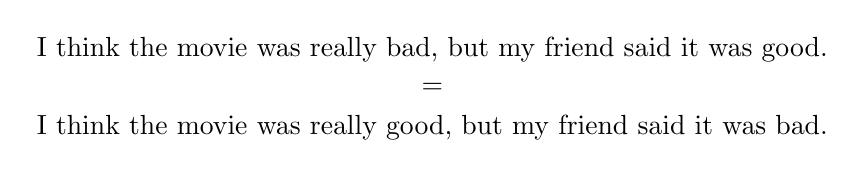
\begin{tikzpicture}
            \node[] at (0, 0) {
                I think the movie was really good, but my friend said it was bad.
            };
            \node[] at (0, 0.5) {
                =
            };
            \node[] at (0, 1) {
                I think the movie was really bad, but my friend said it was good.
            };
        \end{tikzpicture}
    \end{frame}

    \begin{frame}{Word2vec}
        Word2vec: Model words by vectors that encode their semantic content
        \begin{itemize}
            \item Main advantage: Models semantic meaning, allowing us to do mathematics with language
            \item Main disadvantage: Does not consider the structure innate to language
        \end{itemize}
    \end{frame}

    \section{Recurrent neural networks}

    \newcommand{\rnn}[1]{
        \begin{tikzpicture}
            \node[] at (0, 0) {};
            \node[] at (8, 5) {};

            \node[inner sep=0pt, minimum size=11pt, fill=teal!50, circle, draw=black] (n00) at (1, 4) {};
            \node[inner sep=0pt, minimum size=11pt, fill=teal!50, circle, draw=black] (n01) at (1.857, 4) {};
            \node[inner sep=0pt, minimum size=11pt, fill=teal!50, circle, draw=black] (n02) at (2.714, 4) {};
            \ifnum#1<3
                \node[inner sep=0pt, minimum size=11pt, fill=teal!50, circle, draw=black] (n03) at (3.571, 4) {};
            \fi
            \ifnum#1=3
                \node[inner sep=0pt, minimum size=11pt, fill=red!50, circle, draw=red] (n03) at (3.571, 4) {};
            \fi
            \node[inner sep=0pt, minimum size=11pt, fill=teal!50, circle, draw=black] (n04) at (4.429, 4) {};
            \node[inner sep=0pt, minimum size=11pt, fill=teal!50, circle, draw=black] (n05) at (5.286, 4) {};
            \ifnum#1<3
                \node[inner sep=0pt, minimum size=11pt, fill=teal!50, circle, draw=black] (n06) at (6.143, 4) {};
            \fi
            \ifnum#1=3
                \node[inner sep=0pt, minimum size=11pt, fill=red!50, circle, draw=red] (n06) at (6.143, 4) {};
            \fi
            \node[inner sep=0pt, minimum size=11pt, fill=teal!50, circle, draw=black] (n07) at (7, 4) {};

            \ifnum#1=1
                \node[inner sep=0pt, minimum size=11pt, fill=teal!50, circle, draw=black] (n10) at (2, 2.5) {};
                \node[inner sep=0pt, minimum size=11pt, fill=teal!50, circle, draw=black] (n11) at (3.33, 2.5) {};
                \node[inner sep=0pt, minimum size=11pt, fill=teal!50, circle, draw=black] (n12) at (4.66, 2.5) {};
                \node[inner sep=0pt, minimum size=11pt, fill=teal!50, circle, draw=black] (n13) at (6, 2.5) {};

                \node[inner sep=0pt, minimum size=11pt, fill=teal!50, circle, draw=black] (n20) at (4, 1) {};

                \draw[-stealth] (n00) -- (n10);
                \draw[-stealth] (n00) -- (n11);
                \draw[-stealth] (n00) -- (n12);
                \draw[-stealth] (n00) -- (n13);
                \draw[-stealth] (n01) -- (n10);
                \draw[-stealth] (n01) -- (n11);
                \draw[-stealth] (n01) -- (n12);
                \draw[-stealth] (n01) -- (n13);
                \draw[-stealth] (n02) -- (n10);
                \draw[-stealth] (n02) -- (n11);
                \draw[-stealth] (n02) -- (n12);
                \draw[-stealth] (n02) -- (n13);
                \draw[-stealth] (n03) -- (n10);
                \draw[-stealth] (n03) -- (n11);
                \draw[-stealth] (n03) -- (n12);
                \draw[-stealth] (n03) -- (n13);
                \draw[-stealth] (n04) -- (n10);
                \draw[-stealth] (n04) -- (n11);
                \draw[-stealth] (n04) -- (n12);
                \draw[-stealth] (n04) -- (n13);
                \draw[-stealth] (n05) -- (n10);
                \draw[-stealth] (n05) -- (n11);
                \draw[-stealth] (n05) -- (n12);
                \draw[-stealth] (n05) -- (n13);
                \draw[-stealth] (n06) -- (n10);
                \draw[-stealth] (n06) -- (n11);
                \draw[-stealth] (n06) -- (n12);
                \draw[-stealth] (n06) -- (n13);
                \draw[-stealth] (n07) -- (n10);
                \draw[-stealth] (n07) -- (n11);
                \draw[-stealth] (n07) -- (n12);
                \draw[-stealth] (n07) -- (n13);

                \draw[-stealth] (n10) -- (n20);
                \draw[-stealth] (n11) -- (n20);
                \draw[-stealth] (n12) -- (n20);
                \draw[-stealth] (n13) -- (n20);
            \fi

            \ifnum#1>1
                \node[inner sep=0pt, minimum size=11pt, fill=teal!50, circle, draw=black] (n10) at (1.425, 3) {};
                \node[inner sep=0pt, minimum size=11pt, fill=teal!50, circle, draw=black] (n12) at (4.857, 3) {};
                \ifnum#1<3
                    \node[inner sep=0pt, minimum size=11pt, fill=teal!50, circle, draw=black] (n11) at (3.142, 3) {};
                    \node[inner sep=0pt, minimum size=11pt, fill=teal!50, circle, draw=black] (n13) at (6.5715, 3) {};
                    \node[inner sep=0pt, minimum size=11pt, fill=teal!50, circle, draw=black] (n20) at (2.2835, 2) {};
                    \node[inner sep=0pt, minimum size=11pt, fill=teal!50, circle, draw=black] (n21) at (5.714, 2) {};
                    \node[inner sep=0pt, minimum size=11pt, fill=teal!50, circle, draw=black] (n30) at (4, 1) {};
                    \draw[-stealth] (n03) -- (n11);
                    \draw[-stealth] (n06) -- (n13);
                    \draw[-stealth] (n11) -- (n20);
                    \draw[-stealth] (n13) -- (n21);
                    \draw[-stealth] (n20) -- (n30);
                    \draw[-stealth] (n21) -- (n30);
                \fi
                \ifnum#1=3
                    \node[inner sep=0pt, minimum size=11pt, fill=red!50, circle, draw=red] (n11) at (3.142, 3) {};
                    \node[inner sep=0pt, minimum size=11pt, fill=red!50, circle, draw=red] (n13) at (6.5715, 3) {};
                    \node[inner sep=0pt, minimum size=11pt, fill=red!50, circle, draw=red] (n20) at (2.2835, 2) {};
                    \node[inner sep=0pt, minimum size=11pt, fill=red!50, circle, draw=red] (n21) at (5.714, 2) {};
                    \node[inner sep=0pt, minimum size=11pt, fill=red!50, circle, draw=red] (n30) at (4, 1) {};
                    \draw[-stealth,red] (n03) -- (n11);
                    \draw[-stealth,red] (n06) -- (n13);
                    \draw[-stealth,red] (n11) -- (n20);
                    \draw[-stealth,red] (n13) -- (n21);
                    \draw[-stealth,red] (n20) -- (n30);
                    \draw[-stealth,red] (n21) -- (n30);
                \fi

                \draw[-stealth] (n00) -- (n10);
                \draw[-stealth] (n01) -- (n10);
                \draw[-stealth] (n02) -- (n11);
                \draw[-stealth] (n04) -- (n12);
                \draw[-stealth] (n05) -- (n12);
                \draw[-stealth] (n07) -- (n13);

                \draw[-stealth] (n10) -- (n20);
                \draw[-stealth] (n12) -- (n21);

            \fi
        \end{tikzpicture}
    }

    \newsavebox{\rnnann}
    \sbox{\rnnann}{%
        \rnn{1}
    }
    \newsavebox{\rnncnn}
    \sbox{\rnncnn}{%
        \rnn{2}
    }
    \newsavebox{\rnnhighlightedcnn}
    \sbox{\rnnhighlightedcnn}{%
        \rnn{3}
    }

    \newcommand{\drawrnn}[1]{
        \begin{tikzpicture}
            % We start by placing the blocks
            \node[] at (0, 2.3) {};
            \node [
                rectangle,
                minimum width=4cm,
                minimum height=3cm,fill=gray!20,
                rounded corners=0.3cm,
                draw=gray!50,
                label=above:{\small{RNN cell}},
                anchor=north
            ] (rnn) at (0, 0) {};
            \node[anchor=east] at ($ (rnn.north west) - (1, 0.75) $) (stprev){\footnotesize{$state_{t-1}$}};
            \node[anchor=north] at ($ (rnn.south west) - (-1.5, 0.75) $) (it){\footnotesize{$input_{t}$}};
            \node[anchor=west] at ($ (rnn.north east) - (-1, 0.75) $) (st){\footnotesize{$state_{t}$}};
            \node[circle, draw=black,fill=teal!50, text depth=0] (join) at ($ (rnn.north west) - (-1.5, 0.75) $) {$+$};
            \node[fill=orange!50,draw=black] (f) at ($ (join.east) + (1, 0) $) {$f$};
            \node[fill=orange!50, draw=black] (fs) at ($ (join) - (1, 0) $) {$f_s$};
            \node[fill=orange!50, draw=black] (fi) at ($ (join) - (0, 1) $) {$f_i$};
            \draw[-] (stprev) -- (fs);
            \draw[-stealth] (fs) -- (join);
            \draw[-] (it) -- (fi);
            \draw[-stealth] (fi) -- (join);
            \draw[-] (join) -- (f);
            \draw[-stealth] (f) -- (st);

            \ifnum#1>1
                \draw[-stealth] (st) to [in=90, out=90] (stprev);
            \fi
            \ifnum#1=3
                \node[anchor=north west] (out) at ($ (st.south west) + (0, -1) $) {\footnotesize{$output_i$}};
                \draw[] ($ (f) + (0.5, 0) $) to [out=0, in=90] ($ (f) + (0.75, -0.5) $);
                \draw[-stealth] ($ (f) + (0.75, -0.5) $) to [out=270, in=180] (out);
            \fi
        \end{tikzpicture}
    }

    \newsavebox{\rnncell}
    \sbox{\rnncell}{%
        \drawrnn{1}
    }

    \newsavebox{\rnnrecursive}
    \sbox{\rnnrecursive}{%
        \drawrnn{2}
    }
    \newsavebox{\rnnoutput}
    \sbox{\rnnoutput}{%
        \drawrnn{3}
    }

    \newsavebox{\lstmcell}
    \sbox{\lstmcell}{%
        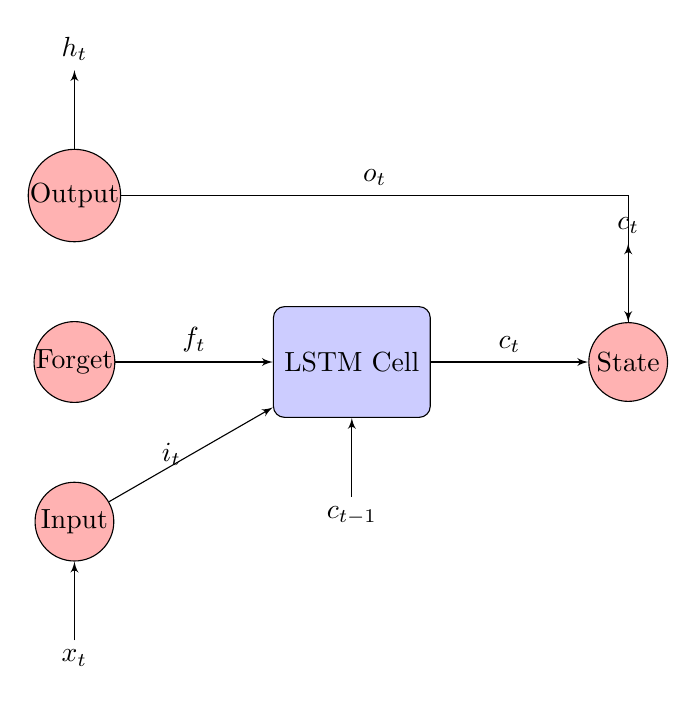
\begin{tikzpicture}
            % Define styles
            \tikzset{
                block/.style={rectangle, draw, fill=blue!20, text width=5em, text centered, rounded corners, minimum height=4em},
                gate/.style={circle, draw, fill=red!30, minimum size=1cm, inner sep=0pt},
                line/.style={draw, -latex'}
            }

            % Place nodes
            \node[block] (cell) {LSTM Cell};
            \node[gate, left=of cell, xshift=-1cm] (forget) {Forget};
            \node[gate, below=of forget] (input) {Input};
            \node[gate, above=of forget] (output) {Output};
            \node[gate, right=of cell, xshift=1cm] (state) {State};

            % Draw connections
            \draw[line] (forget) -- node[midway, above] {$f_t$} (cell);
            \draw[line] (input) -- node[midway, left] {$i_t$} (cell);
            \draw[line] (cell) -- node[midway, above] {$c_t$} (state);
            \draw[line] (output) -| node[near start, above] {$o_t$} (state);

            % Connection for previous and next cell states
            \node[below=of cell] (prev_ct) {$c_{t-1}$};
            \node[above=of state] (next_ct) {$c_{t}$};
            \draw[line] (prev_ct) -- (cell);
            \draw[line] (state) -- (next_ct);

            % Input and output connections
            \node[below=of input] (xt) {$x_{t}$};
            \node[above=of output] (ht) {$h_{t}$};
            \draw[line] (xt) -- (input);
            \draw[line] (output) -- (ht);

        \end{tikzpicture}
    }

    \begin{frame}{Recurrent neural networks}
        \only<1-19>{
            \begin{tikzpicture}
                \node[] at (0, 0) {};
                \node[] at (10, 7) {};

                \only<1-2,4-5,7-12>{
                    \node[] at (5, 6) {
                        I think the movie had a great plot
                    };
                }
                \only<2>{
                    \draw[-stealth] (2.42, 5.85) -- (2, 4.7);
                    \draw[-stealth] (2.97, 5.85) -- (2.83, 4.7);
                    \draw[-stealth] (3.7, 5.85) -- (3.65, 4.7);
                    \draw[-stealth] (4.6, 5.85) -- (4.52, 4.7);
                    \draw[-stealth] (5.45, 5.85) -- (5.38, 4.7);
                    \draw[-stealth] (5.93, 5.85) -- (6.2, 4.7);
                    \draw[-stealth] (6.5, 5.85) -- (7.05, 4.7);
                    \draw[-stealth] (7.3, 5.85) -- (7.9, 4.7);
                }
                \only<2-3>{
                    \node[] at (5, 3) {
                        \usebox{\rnnann}
                    };
                    \only<2>{
                        \node[] (out) at (4.95, 0.6) {Positive};
                    }
                    \only<3>{
                        \node[] (out) at (4.95, 0.6) {?};
                    }
                    \draw[-stealth] (4.95, 1.3) -- (out);
                }
                \only<3>{
                    \node[] at (5, 6) {
                        The movie had a great plot I think
                    };
                    \draw[-stealth] (2.6, 5.85) -- (2, 4.7);
                    \draw[-stealth] (3.5, 5.85) -- (2.83, 4.7);
                    \draw[-stealth] (4.35, 5.85) -- (3.65, 4.7);
                    \draw[-stealth] (4.85, 5.85) -- (4.52, 4.7);
                    \draw[-stealth] (5.45, 5.85) -- (5.38, 4.7);
                    \draw[-stealth] (6.25, 5.85) -- (6.2, 4.7);
                    \draw[-stealth] (6.7, 5.85) -- (7.05, 4.7);
                    \draw[-stealth] (7.3, 5.85) -- (7.9, 4.7);
                }
                \only<5>{
                    \node[] at (5, 3) {
                        \usebox{\rnncnn}
                    };

                    \draw[-stealth] (2.42, 5.85) -- (2, 4.7);
                    \draw[-stealth] (2.97, 5.85) -- (2.83, 4.7);
                    \draw[-stealth] (3.7, 5.85) -- (3.65, 4.7);
                    \draw[-stealth] (4.6, 5.85) -- (4.52, 4.7);
                    \draw[-stealth] (5.45, 5.85) -- (5.38, 4.7);
                    \draw[-stealth] (5.93, 5.85) -- (6.2, 4.7);
                    \draw[-stealth] (6.5, 5.85) -- (7.05, 4.7);
                    \draw[-stealth] (7.3, 5.85) -- (7.9, 4.7);

                    \draw[-stealth] (4.95, 1.3) -- (out);
                    \node[] (out) at (4.95, 0.6) {Positive};
                }
                \only<6>{
                    \node[] at (5, 6) {
                        I think the \textcolor{red}{movie} had a \textcolor{red}{great} plot
                    };
                    \draw[-stealth] (2.42, 5.85) -- (2, 4.7);
                    \draw[-stealth] (2.97, 5.85) -- (2.83, 4.7);
                    \draw[-stealth] (3.7, 5.85) -- (3.65, 4.7);
                    \draw[-stealth, red] (4.6, 5.85) -- (4.52, 4.7);
                    \draw[-stealth] (5.45, 5.85) -- (5.38, 4.7);
                    \draw[-stealth] (5.93, 5.85) -- (6.2, 4.7);
                    \draw[-stealth, red] (6.5, 5.85) -- (7.05, 4.7);
                    \draw[-stealth] (7.3, 5.85) -- (7.9, 4.7);
                    \node[] at (5, 3) {
                        \usebox{\rnnhighlightedcnn}
                    };

                    \draw[-stealth,red] (4.95, 1.3) -- (out);
                    \node[red] (out) at (4.95, 0.6) {Positive};
                }
                \only<8-12>{
                    \onslide<8->{
                        \node[fill=gray!25,draw=gray!50] (s0) at (1, 3) {...};
                        \draw[-stealth] (2.42, 5.85) -- (s0.north);
                    }
                    \onslide<9->{
                        \node[fill=gray!25,draw=gray!50] (s1) at (2.14, 3) {...};
                        \draw[-stealth] (2.97, 5.85) -- (s1.north);
                        \draw[-stealth] (s0) -- (s1);
                    }
                    \onslide<10->{
                        \node[fill=gray!25,draw=gray!50] (s2) at (3.28, 3) {...};
                        \draw[-stealth] (3.7, 5.85) -- (s2.north);
                        \draw[-stealth] (s1) -- (s2);
                    }
                    \only<11-12>{
                        \node[fill=gray!25,draw=gray!50] (s3) at (4.42, 3) {...};
                        \node[fill=gray!25,draw=gray!50] (s4) at (5.57, 3) {...};
                        \node[fill=gray!25,draw=gray!50] (s5) at (6.71, 3) {...};
                        \node[fill=gray!25,draw=gray!50] (s6) at (7.85, 3) {...};
                        \node[fill=gray!25,draw=gray!50] (s7) at (9, 3) {...};
                        \draw[-stealth] (4.6, 5.85) -- (s3.north);
                        \draw[-stealth] (5.45, 5.85) -- (s4.north);
                        \draw[-stealth] (5.93, 5.85) -- (s5.north);
                        \draw[-stealth] (6.5, 5.85) -- (s6.north);
                        \draw[-stealth] (7.3, 5.85) -- (s7.north);
                        \draw[-stealth] (s2) -- (s3);
                        \draw[-stealth] (s3) -- (s4);
                        \draw[-stealth] (s4) -- (s5);
                        \draw[-stealth] (s5) -- (s6);
                        \draw[-stealth] (s6) -- (s7);
                    }
                    \only<12>{
                        \node[] (out) at (9, 2) {Positive};
                        \draw[-stealth] (s7) -- (out);
                    }
                }
                \only<13>{
                    \node[] at (5, 3.5) {
                        \usebox{\rnncell}
                    };
                }
                \only<14>{
                    \node[] at (5, 3.5) {
                        \usebox{\rnnrecursive}
                    };
                }
                \only<15>{
                    \node[] at (5, 3.5) {
                        Blackboard demo!
                    };
                }
                \only<16>{
                    \node[] at (5, 3.5) {
                        \usebox{\rnnoutput}
                    };
                }
                \only<17>{
                    \node[] at (5, 3.5) {
                        More blackboard demo!
                    };
                }
                \only<18>{
                    \node[inner sep=0pt, draw=black] at (5, 3.5) {
                        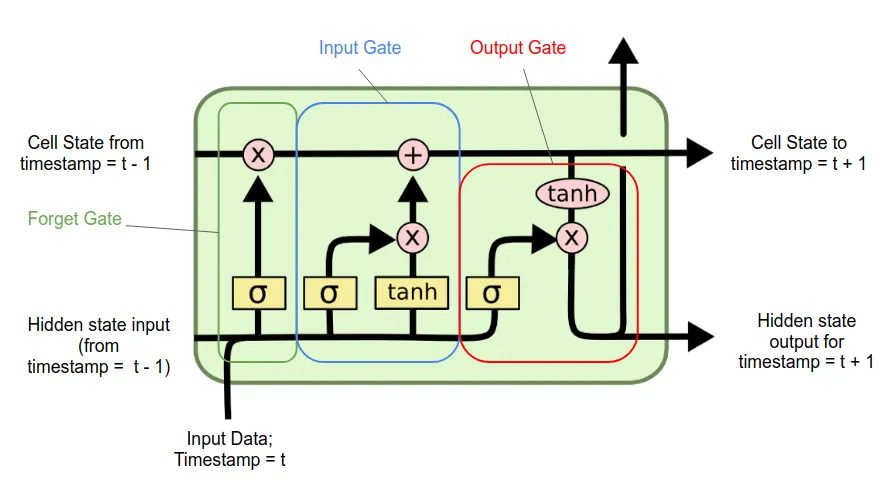
\includegraphics[width=7cm]{data/lstm.png}
                    };

                }
                \only<19>{
                    \node[] at (5, 3.5) {
                        {\tiny
                            \url{https://www.tensorflow.org/guide/keras/working_with_rnns}
                        }
                    };
                }
            \end{tikzpicture}
        }
        \only<20>{
            RNNs: Models sequences by recursively considering what it has seen so far, and what the new input token is
            \begin{itemize}
                \item Main advantage: Is able to encompass both long- and short-term dependencies
                \item Main disadvantage: In practice it is hard to weigh long-term versus short-term
            \end{itemize}
        }
    \end{frame}

    \section{Transformers}

    \begin{frame}[t]{Transformers}
        \begin{tikzpicture}
            \node[] at (0, 0) {};
            \node[] at (10, 7) {};

            \visible<1>{
                \node[inner sep=0pt, draw=black] at (5, 3.2) {
                    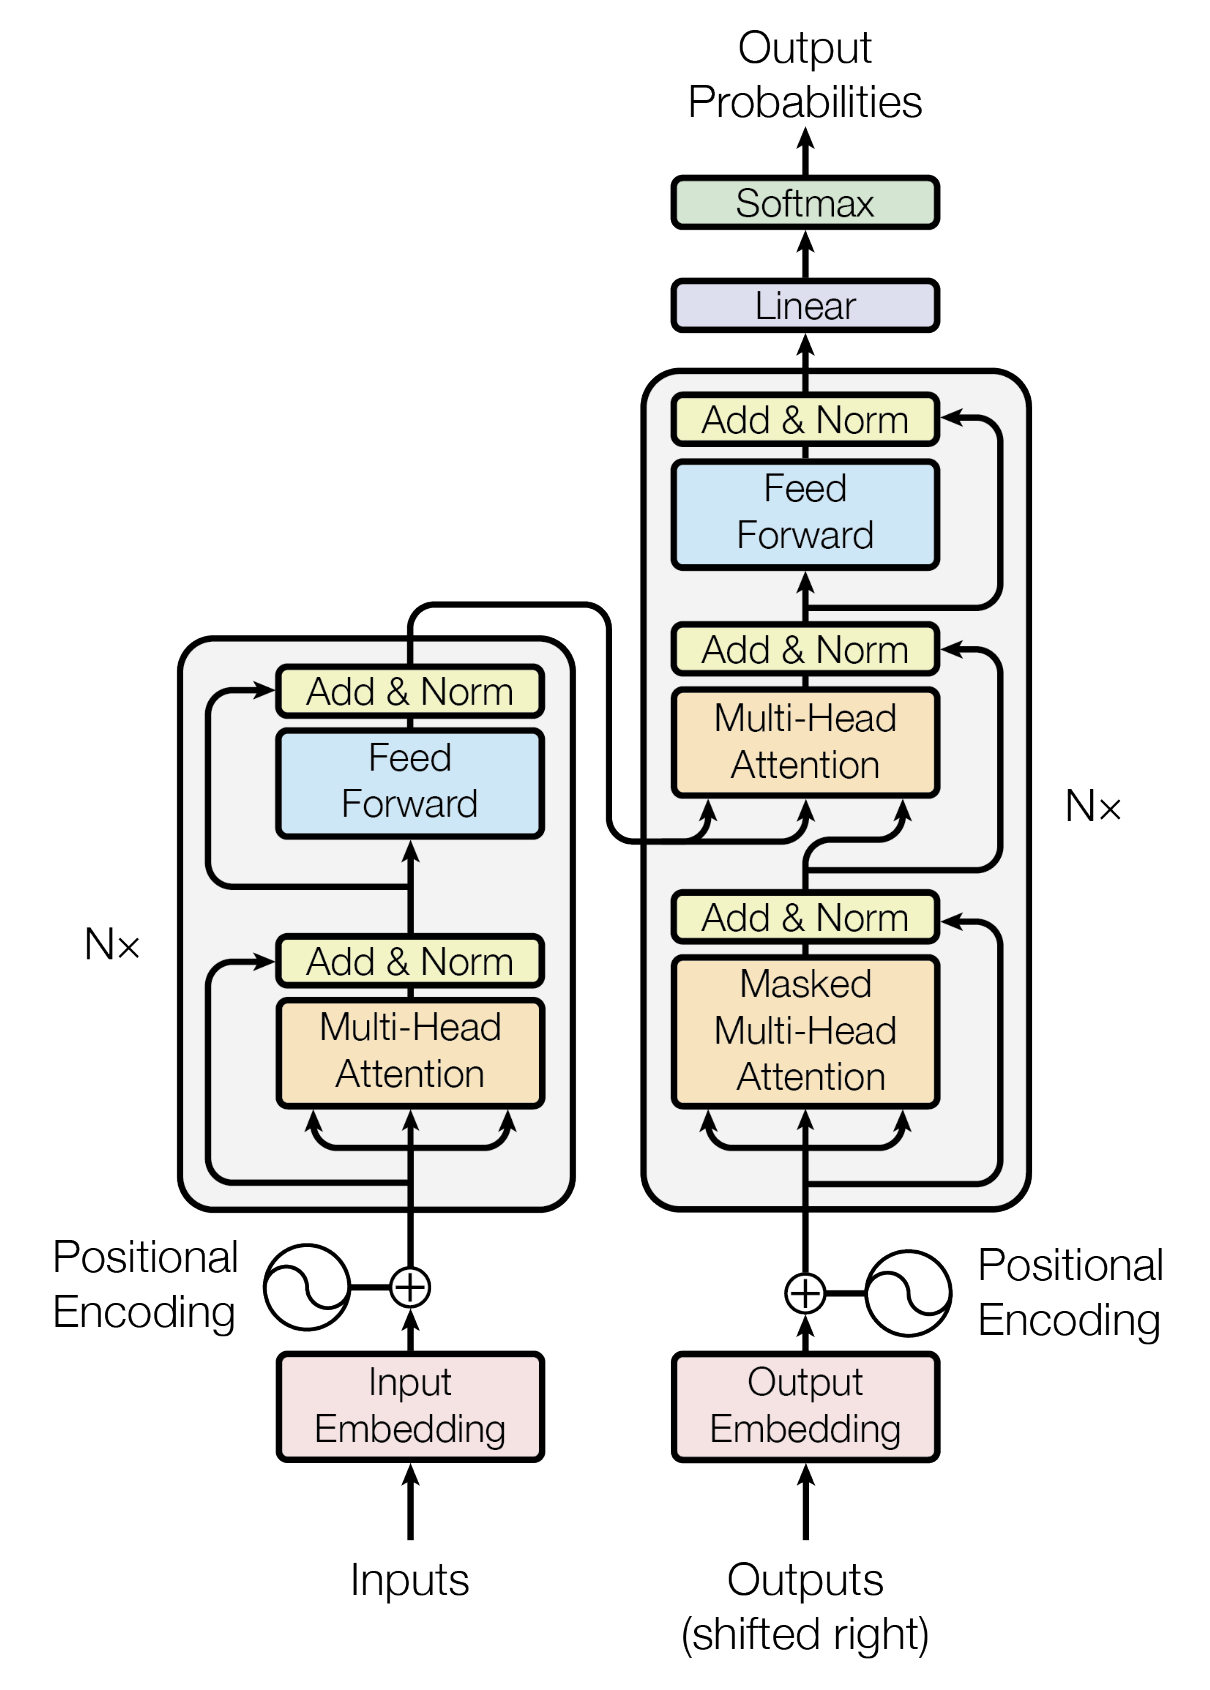
\includegraphics[width=4cm]{data/transformer.png}
                };
            }
            \visible<2>{
                \node[text width=10.5cm] at (5, 3.2) {
                    Auto-regression: The model generates one token at a time, based on the tokens it has generated so far
                };
            }
        \end{tikzpicture}
    \end{frame}
    \begin{frame}{Transformers: Attention}
        \begin{tikzpicture}
            \node[] at (0, 0) {};
            \node[] at (10, 7) {};

                \only<1,13-16>{
                    \node[] at (4, 6) {
                        The movie was great, the actors were
                    };
                }
                \only<2,8>{
                    \node[] at (4, 6) {
                        The movie was \textcolor{red}{great}, the actors were
                    };
                }
                \only<1-9,13-16>{
                    \draw[black] (6.9, 5.8) -- (8.2, 5.8);
                }
                \only<3>{
                    \node[] at (4, 6) {
                        \textcolor{gray!20}{The movie was great, the actors were}
                    };
                }
                \only<4>{
                    \node[] at (4, 6) {
                        The \textcolor{gray!20}{movie was great, the actors were}
                    };
                }
                \only<5>{
                    \node[] at (4, 6) {
                        The movie \textcolor{gray!20}{was great, the actors were}
                    };
                }
                \only<6>{
                    \node[] at (4, 6) {
                        The movie was \textcolor{gray!20}{great, the actors were}
                    };
                }
                \only<7>{
                    \node[] at (4, 6) {
                        The movie was \textcolor{red}{great}\textcolor{gray!20}{, the actors were}
                    };
                }
                \only<9>{
                    \node[] at (4, 6) {
                        The \textcolor{red!70!black}{movie} was \textcolor{red!70!black}{great}, the \textcolor{red!70!black}{actors} were
                    };
                }
                \only<10>{
                    \node[anchor=north,align=center] at (4.7, 6.3) {
                        The \textcolor{red!40!black}{movie} was \textcolor{red!40!black}{great}, we saw it at the new\\
                        \textcolor{red!60!black}{Cinema} in the \textcolor{red!65!black}{city center}, right down by the\\
                        restaurant where we went for my \textcolor{red!75!black}{birthday} that\\
                        one year, the one where the \textcolor{red!85!black}{clown} was\\
                        inside the \textcolor{red!90!black}{cake}, the \textcolor{red!95!black}{actors} were \textcolor{black!2}{awesome}
                    };
                    \draw[black] (6.5, 3.9) -- (7.8, 3.9);
                }
                \only<11>{
                    \node[anchor=north,align=center] at (4.7, 6.3) {
                        The \textcolor{red!90!black}{movie} was \textcolor{red!90!black}{great}, we saw it at the new\\
                        \textcolor{red!90!black}{Cinema} in the \textcolor{red!90!black}{city center}, right down by the\\
                        restaurant where we went for my \textcolor{red!90!black}{birthday} that\\
                        one year, the one where the \textcolor{red!90!black}{clown} was\\
                        inside the \textcolor{red!90!black}{cake}, the \textcolor{red!90!black}{actors} were \textcolor{black!2}{awesome}
                    };
                    \draw[black] (6.5, 3.9) -- (7.8, 3.9);
                }
                \only<12>{
                    \node[anchor=north,align=center] at (4.7, 6.3) {
                        The \textcolor{purple!90!black}{movie} was \textcolor{red!90!black}{great}, we saw it at the new\\
                        \textcolor{green!90!black}{Cinema} in the \textcolor{green!90!black}{city center}, right down by the\\
                        restaurant where we went for my \textcolor{blue!90!black}{birthday} that\\
                        one year, the one where the \textcolor{blue!90!black}{clown} was\\
                        inside the \textcolor{blue!90!black}{cake}, the \textcolor{purple!90!black}{actors} were \textcolor{black!2}{awesome}
                    };
                    \draw[black] (6.5, 3.9) -- (7.8, 3.9);
                }
                \only<14-16>{
                    \node[] at (1.2, 5.2) {[};
                    \node[] at (1.37, 5.2) {8};
                    \node[] at (2.25, 5.2) {7};
                    \node[] at (3.1, 5.2) {9};
                    \node[] at (3.9, 5.2) {6};
                    \node[] at (4.33, 5.2) {0};
                    \node[] at (4.72, 5.2) {8};
                    \node[] at (5.55, 5.2) {4};
                    \node[] at (6.5, 5.2) {10};
                    \node[] at (6.75, 5.2) {]};

                    \draw[-stealth] (7, 5.2) -- (7.3, 5.2);
                    \node[] at (7.55, 5.2) {?};
                }
                \only<15-16>{
                    \node[] at (1.2, 4.5) {[};
                    \node[] at (1.37, 4.5) {0};
                    \node[] at (2.25, 4.5) {0};
                    \node[] at (3.1, 4.5) {0};
                    \node[] at (3.9, 4.5) {1};
                    \node[] at (4.33, 4.5) {0};
                    \node[] at (4.72, 4.5) {0};
                    \node[] at (5.55, 4.5) {0};
                    \node[] at (6.5, 4.5) {0};
                    \node[] at (6.75, 4.5) {]};
                }
                \only<16>{
                    \node[] at (1.2, 3.8) {[};
                    \node[] at (1.37, 3.8) {0};
                    \node[] at (2.25, 3.8) {0};
                    \node[] at (3.1, 3.8) {0};
                    \node[] at (3.9, 3.8) {6};
                    \node[] at (4.33, 3.8) {0};
                    \node[] at (4.72, 3.8) {0};
                    \node[] at (5.55, 3.8) {0};
                    \node[] at (6.5, 3.8) {0};
                    \node[] at (6.75, 3.8) {]};

                    \node[] at (3.975, 4.85) {$\times$};
                    \node[] at (3.975, 4.15) {$=$};
                }

        \end{tikzpicture}
    \end{frame}

    \newcommand{\drawsines}[1]{
        \begin{tikzpicture}
            \begin{axis}[
                domain=-2*pi:2*pi,
                samples=500,
                xmin=-2*pi,
                xmax=2*pi,
                xmajorticks=false,
                ymajorticks=false,
                height=5cm,
                width=9cm,
                ymin=-2,
                ymax=9
            ]
                \addplot[no marks,thick,firstcolor] {7.5 + sin(deg(2*x))};

                \node[fill=firstcolor, circle, inner sep=2pt] at (axis cs: -5.15, 8.3) {};
                \node[fill=firstcolor, circle, inner sep=2pt] at (axis cs: -1.75, 8) {};
                \node[fill=firstcolor, circle, inner sep=2pt] at (axis cs: 1.65, 7.5) {};
                \node[fill=firstcolor, circle, inner sep=2pt] at (axis cs: 5.05, 7) {};

                \ifnum#1>1
                    \addplot[no marks,thick,secondcolor] {5 + sin(deg(3*x))};

                    \node[fill=secondcolor, circle, inner sep=2pt] at (axis cs: -5.15, 4.9) {};
                    \node[fill=secondcolor, circle, inner sep=2pt] at (axis cs: -1.75, 5.9) {};
                    \node[fill=secondcolor, circle, inner sep=2pt] at (axis cs: 1.65, 4.1) {};
                    \node[fill=secondcolor, circle, inner sep=2pt] at (axis cs: 5.05, 5.6) {};

                    \addplot[no marks,thick,thirdcolor] {2.5 + sin(deg(5*x))};

                    \node[fill=thirdcolor, circle, inner sep=2pt] at (axis cs: -5.15, 2.1) {};
                    \node[fill=thirdcolor, circle, inner sep=2pt] at (axis cs: -1.75, 1.8) {};
                    \node[fill=thirdcolor, circle, inner sep=2pt] at (axis cs: 1.65, 3.4) {};
                    \node[fill=thirdcolor, circle, inner sep=2pt] at (axis cs: 5.05, 2.8) {};

                    \addplot[no marks,thick,fourthcolor] {sin(deg(7*x))};

                    \node[fill=fourthcolor, circle, inner sep=2pt] at (axis cs: -5.15, 0.9) {};
                    \node[fill=fourthcolor, circle, inner sep=2pt] at (axis cs: -1.75, 0.6) {};
                    \node[fill=fourthcolor, circle, inner sep=2pt] at (axis cs: 1.65, -0.8) {};
                    \node[fill=fourthcolor, circle, inner sep=2pt] at (axis cs: 5.05, -0.4) {};
                \fi
            \end{axis}
        \end{tikzpicture}
    }

    \newsavebox{\firstsine}
    \sbox{\firstsine}{%
        \drawsines{1}
    }
    \newsavebox{\allsines}
    \sbox{\allsines}{%
        \drawsines{2}
    }

    \begin{frame}{Transformers: Positional encoding}
        \begin{tikzpicture}
            \node[] at (0, 0) {};
            \node[] at (10, 7) {};
            \def\nodesize{12pt}

            \only<1-7>{
                \node[anchor=north] at (5, 6.5) {
                    The movie was great.
                };
            }
            \only<2-7>{
                \node[] (the) at (2, 5) {the};
                \node[] (movie) at (4, 5) {movie};
                \node[] (was) at (6, 5) {was};
                \node[] (great) at (8, 5) {great};
                \draw[-stealth] (3.6, 6) -- (the.north);
                \draw[-stealth] (4.5, 6) -- (movie.north);
                \draw[-stealth] (5.5, 6) -- (was.north);
                \draw[-stealth] (6.2, 6) -- (great.north);
            };
            \only<3-7>{
                \node[] (theidx) at (2, 4) {4};
                \node[] (movieidx) at (4, 4) {17};
                \node[] (wasidx) at (6, 4) {91};
                \node[] (greatidx) at (8, 4) {52};
                \draw[-stealth] (the) -- (theidx.north);
                \draw[-stealth] (movie) -- (movieidx.north);
                \draw[-stealth] (was) -- (wasidx.north);
                \draw[-stealth] (great) -- (greatidx.north);
            };
            \only<4-7>{
                \node[draw=black, minimum width=\nodesize, minimum height=\nodesize, inner sep=0pt, outer sep=0pt] (n00) at (2, 3) {\tiny{0.5}};
                \node[draw=black, minimum width=\nodesize, minimum height=\nodesize, inner sep=0pt, outer sep=0pt, anchor=north] (n10) at (n00.south) {\tiny{0.3}};
                \node[draw=black, minimum width=\nodesize, minimum height=\nodesize, inner sep=0pt, outer sep=0pt, anchor=north] (n20) at (n10.south) {\tiny{0.7}};
                \node[draw=black, minimum width=\nodesize, minimum height=\nodesize, inner sep=0pt, outer sep=0pt, anchor=north] (n30) at (n20.south) {\tiny{0.0}};

                \node[draw=black, minimum width=\nodesize, minimum height=\nodesize, inner sep=0pt, outer sep=0pt] (n01) at (4, 3) {\tiny{0.2}};
                \node[draw=black, minimum width=\nodesize, minimum height=\nodesize, inner sep=0pt, outer sep=0pt, anchor=north] (n11) at (n01.south) {\tiny{0.0}};
                \node[draw=black, minimum width=\nodesize, minimum height=\nodesize, inner sep=0pt, outer sep=0pt, anchor=north] (n21) at (n11.south) {\tiny{1.0}};
                \node[draw=black, minimum width=\nodesize, minimum height=\nodesize, inner sep=0pt, outer sep=0pt, anchor=north] (n31) at (n21.south) {\tiny{0.3}};

                \node[draw=black, minimum width=\nodesize, minimum height=\nodesize, inner sep=0pt, outer sep=0pt] (n02) at (6, 3) {\tiny{1.0}};
                \node[draw=black, minimum width=\nodesize, minimum height=\nodesize, inner sep=0pt, outer sep=0pt, anchor=north] (n12) at (n02.south) {\tiny{0.1}};
                \node[draw=black, minimum width=\nodesize, minimum height=\nodesize, inner sep=0pt, outer sep=0pt, anchor=north] (n22) at (n12.south) {\tiny{0.2}};
                \node[draw=black, minimum width=\nodesize, minimum height=\nodesize, inner sep=0pt, outer sep=0pt, anchor=north] (n32) at (n22.south) {\tiny{0.8}};

                \node[draw=black, minimum width=\nodesize, minimum height=\nodesize, inner sep=0pt, outer sep=0pt] (n03) at (8, 3) {\tiny{0.8}};
                \node[draw=black, minimum width=\nodesize, minimum height=\nodesize, inner sep=0pt, outer sep=0pt, anchor=north] (n13) at (n03.south) {\tiny{0.4}};
                \node[draw=black, minimum width=\nodesize, minimum height=\nodesize, inner sep=0pt, outer sep=0pt, anchor=north] (n23) at (n13.south) {\tiny{0.2}};
                \node[draw=black, minimum width=\nodesize, minimum height=\nodesize, inner sep=0pt, outer sep=0pt, anchor=north] (n33) at (n23.south) {\tiny{0.6}};

                \draw[-stealth] (theidx) -- (n00);
                \draw[-stealth] (movieidx) -- (n01);
                \draw[-stealth] (wasidx) -- (n02);
                \draw[-stealth] (greatidx) -- (n03);
            }
            \only<5>{
                \node[draw=red, minimum width=\nodesize, minimum height=\nodesize, inner sep=0pt, outer sep=0pt, anchor=west, red] (p00) at (n00.east) {};
                \node[draw=red, minimum width=\nodesize, minimum height=\nodesize, inner sep=0pt, outer sep=0pt, anchor=west, red] (p10) at (n10.east) {};
                \node[draw=red, minimum width=\nodesize, minimum height=\nodesize, inner sep=0pt, outer sep=0pt, anchor=west, red] (p20) at (n20.east) {};
                \node[draw=red, minimum width=\nodesize, minimum height=\nodesize, inner sep=0pt, outer sep=0pt, anchor=west, red] (p30) at (n30.east) {};

                \node[draw=red, minimum width=\nodesize, minimum height=\nodesize, inner sep=0pt, outer sep=0pt, anchor=west, red] (p01) at (n01.east) {};
                \node[draw=red, minimum width=\nodesize, minimum height=\nodesize, inner sep=0pt, outer sep=0pt, anchor=west, red] (p11) at (n11.east) {};
                \node[draw=red, minimum width=\nodesize, minimum height=\nodesize, inner sep=0pt, outer sep=0pt, anchor=west, red] (p21) at (n21.east) {};
                \node[draw=red, minimum width=\nodesize, minimum height=\nodesize, inner sep=0pt, outer sep=0pt, anchor=west, red] (p31) at (n31.east) {};

                \node[draw=red, minimum width=\nodesize, minimum height=\nodesize, inner sep=0pt, outer sep=0pt, anchor=west, red] (p02) at (n02.east) {};
                \node[draw=red, minimum width=\nodesize, minimum height=\nodesize, inner sep=0pt, outer sep=0pt, anchor=west, red] (p12) at (n12.east) {};
                \node[draw=red, minimum width=\nodesize, minimum height=\nodesize, inner sep=0pt, outer sep=0pt, anchor=west, red] (p22) at (n22.east) {};
                \node[draw=red, minimum width=\nodesize, minimum height=\nodesize, inner sep=0pt, outer sep=0pt, anchor=west, red] (p32) at (n32.east) {};

                \node[draw=red, minimum width=\nodesize, minimum height=\nodesize, inner sep=0pt, outer sep=0pt, anchor=west, red] (p03) at (n03.east) {};
                \node[draw=red, minimum width=\nodesize, minimum height=\nodesize, inner sep=0pt, outer sep=0pt, anchor=west, red] (p13) at (n13.east) {};
                \node[draw=red, minimum width=\nodesize, minimum height=\nodesize, inner sep=0pt, outer sep=0pt, anchor=west, red] (p23) at (n23.east) {};
                \node[draw=red, minimum width=\nodesize, minimum height=\nodesize, inner sep=0pt, outer sep=0pt, anchor=west, red] (p33) at (n33.east) {};
            }
            \only<6>{
                \node[draw=red, minimum width=\nodesize, minimum height=\nodesize, inner sep=0pt, outer sep=0pt, anchor=west, red, red, font=\tiny] (p00) at (n00.east) {0};
                \node[draw=red, minimum width=\nodesize, minimum height=\nodesize, inner sep=0pt, outer sep=0pt, anchor=west, red, red, font=\tiny] (p10) at (n10.east) {0};
                \node[draw=red, minimum width=\nodesize, minimum height=\nodesize, inner sep=0pt, outer sep=0pt, anchor=west, red, red, font=\tiny] (p20) at (n20.east) {0};
                \node[draw=red, minimum width=\nodesize, minimum height=\nodesize, inner sep=0pt, outer sep=0pt, anchor=west, red, red, font=\tiny] (p30) at (n30.east) {0};

                \node[draw=red, minimum width=\nodesize, minimum height=\nodesize, inner sep=0pt, outer sep=0pt, anchor=west, red, red, font=\tiny] (p01) at (n01.east) {1};
                \node[draw=red, minimum width=\nodesize, minimum height=\nodesize, inner sep=0pt, outer sep=0pt, anchor=west, red, red, font=\tiny] (p11) at (n11.east) {1};
                \node[draw=red, minimum width=\nodesize, minimum height=\nodesize, inner sep=0pt, outer sep=0pt, anchor=west, red, red, font=\tiny] (p21) at (n21.east) {1};
                \node[draw=red, minimum width=\nodesize, minimum height=\nodesize, inner sep=0pt, outer sep=0pt, anchor=west, red, red, font=\tiny] (p31) at (n31.east) {1};

                \node[draw=red, minimum width=\nodesize, minimum height=\nodesize, inner sep=0pt, outer sep=0pt, anchor=west, red, red, font=\tiny] (p02) at (n02.east) {2};
                \node[draw=red, minimum width=\nodesize, minimum height=\nodesize, inner sep=0pt, outer sep=0pt, anchor=west, red, red, font=\tiny] (p12) at (n12.east) {2};
                \node[draw=red, minimum width=\nodesize, minimum height=\nodesize, inner sep=0pt, outer sep=0pt, anchor=west, red, red, font=\tiny] (p22) at (n22.east) {2};
                \node[draw=red, minimum width=\nodesize, minimum height=\nodesize, inner sep=0pt, outer sep=0pt, anchor=west, red, red, font=\tiny] (p32) at (n32.east) {3};

                \node[draw=red, minimum width=\nodesize, minimum height=\nodesize, inner sep=0pt, outer sep=0pt, anchor=west, red, red, font=\tiny] (p03) at (n03.east) {3};
                \node[draw=red, minimum width=\nodesize, minimum height=\nodesize, inner sep=0pt, outer sep=0pt, anchor=west, red, red, font=\tiny] (p13) at (n13.east) {3};
                \node[draw=red, minimum width=\nodesize, minimum height=\nodesize, inner sep=0pt, outer sep=0pt, anchor=west, red, red, font=\tiny] (p23) at (n23.east) {3};
                \node[draw=red, minimum width=\nodesize, minimum height=\nodesize, inner sep=0pt, outer sep=0pt, anchor=west, red, font=\tiny] (p33) at (n33.east) {3};
            }
            \only<7>{
                \node[draw=red, minimum width=\nodesize, minimum height=\nodesize, inner sep=0pt, outer sep=0pt, anchor=west, red, red, font=\tiny] (p00) at (n00.east) {0};
                \node[draw=red, minimum width=\nodesize, minimum height=\nodesize, inner sep=0pt, outer sep=0pt, anchor=west, red, red, font=\tiny] (p10) at (n10.east) {0};
                \node[draw=red, minimum width=\nodesize, minimum height=\nodesize, inner sep=0pt, outer sep=0pt, anchor=west, red, red, font=\tiny] (p20) at (n20.east) {0};
                \node[draw=red, minimum width=\nodesize, minimum height=\nodesize, inner sep=0pt, outer sep=0pt, anchor=west, red, red, font=\tiny] (p30) at (n30.east) {0};

                \node[draw=red, minimum width=\nodesize, minimum height=\nodesize, inner sep=0pt, outer sep=0pt, anchor=west, red, red, font=\tiny] (p01) at (n01.east) {0.3};
                \node[draw=red, minimum width=\nodesize, minimum height=\nodesize, inner sep=0pt, outer sep=0pt, anchor=west, red, red, font=\tiny] (p11) at (n11.east) {0.3};
                \node[draw=red, minimum width=\nodesize, minimum height=\nodesize, inner sep=0pt, outer sep=0pt, anchor=west, red, red, font=\tiny] (p21) at (n21.east) {0.3};
                \node[draw=red, minimum width=\nodesize, minimum height=\nodesize, inner sep=0pt, outer sep=0pt, anchor=west, red, red, font=\tiny] (p31) at (n31.east) {0.3};

                \node[draw=red, minimum width=\nodesize, minimum height=\nodesize, inner sep=0pt, outer sep=0pt, anchor=west, red, red, font=\tiny] (p02) at (n02.east) {0.6};
                \node[draw=red, minimum width=\nodesize, minimum height=\nodesize, inner sep=0pt, outer sep=0pt, anchor=west, red, red, font=\tiny] (p12) at (n12.east) {0.6};
                \node[draw=red, minimum width=\nodesize, minimum height=\nodesize, inner sep=0pt, outer sep=0pt, anchor=west, red, red, font=\tiny] (p22) at (n22.east) {0.6};
                \node[draw=red, minimum width=\nodesize, minimum height=\nodesize, inner sep=0pt, outer sep=0pt, anchor=west, red, red, font=\tiny] (p32) at (n32.east) {0.6};

                \node[draw=red, minimum width=\nodesize, minimum height=\nodesize, inner sep=0pt, outer sep=0pt, anchor=west, red, red, font=\tiny] (p03) at (n03.east) {1};
                \node[draw=red, minimum width=\nodesize, minimum height=\nodesize, inner sep=0pt, outer sep=0pt, anchor=west, red, red, font=\tiny] (p13) at (n13.east) {1};
                \node[draw=red, minimum width=\nodesize, minimum height=\nodesize, inner sep=0pt, outer sep=0pt, anchor=west, red, red, font=\tiny] (p23) at (n23.east) {1};
                \node[draw=red, minimum width=\nodesize, minimum height=\nodesize, inner sep=0pt, outer sep=0pt, anchor=west, red, font=\tiny] (p33) at (n33.east) {1};
            }
            \only<8>{
                \node[] at (5.45, 6) {
                    \usebox{\firstsine}
                };
                \node[draw=red, minimum width=\nodesize, minimum height=\nodesize, inner sep=0pt, outer sep=0pt, anchor=west, red,font=\tiny] (p00) at (n00.east) {0.9};
                \node[draw=red, minimum width=\nodesize, minimum height=\nodesize, inner sep=0pt, outer sep=0pt, anchor=west, red,font=\tiny] (p10) at (n10.east) {0.9};
                \node[draw=red, minimum width=\nodesize, minimum height=\nodesize, inner sep=0pt, outer sep=0pt, anchor=west, red,font=\tiny] (p20) at (n20.east) {0.9};
                \node[draw=red, minimum width=\nodesize, minimum height=\nodesize, inner sep=0pt, outer sep=0pt, anchor=west, red,font=\tiny] (p30) at (n30.east) {0.9};

                \node[draw=red, minimum width=\nodesize, minimum height=\nodesize, inner sep=0pt, outer sep=0pt, anchor=west, red,font=\tiny] (p01) at (n01.east) {0.3};
                \node[draw=red, minimum width=\nodesize, minimum height=\nodesize, inner sep=0pt, outer sep=0pt, anchor=west, red,font=\tiny] (p11) at (n11.east) {0.3};
                \node[draw=red, minimum width=\nodesize, minimum height=\nodesize, inner sep=0pt, outer sep=0pt, anchor=west, red,font=\tiny] (p21) at (n21.east) {0.3};
                \node[draw=red, minimum width=\nodesize, minimum height=\nodesize, inner sep=0pt, outer sep=0pt, anchor=west, red,font=\tiny] (p31) at (n31.east) {0.3};

                \node[draw=red, minimum width=\nodesize, minimum height=\nodesize, inner sep=0pt, outer sep=0pt, anchor=west, red,font=\tiny] (p02) at (n02.east) {-0.3};
                \node[draw=red, minimum width=\nodesize, minimum height=\nodesize, inner sep=0pt, outer sep=0pt, anchor=west, red,font=\tiny] (p12) at (n12.east) {-0.3};
                \node[draw=red, minimum width=\nodesize, minimum height=\nodesize, inner sep=0pt, outer sep=0pt, anchor=west, red,font=\tiny] (p22) at (n22.east) {-0.3};
                \node[draw=red, minimum width=\nodesize, minimum height=\nodesize, inner sep=0pt, outer sep=0pt, anchor=west, red,font=\tiny] (p32) at (n32.east) {-0.3};

                \node[draw=red, minimum width=\nodesize, minimum height=\nodesize, inner sep=0pt, outer sep=0pt, anchor=west, red,font=\tiny] (p03) at (n03.east) {-0.9};
                \node[draw=red, minimum width=\nodesize, minimum height=\nodesize, inner sep=0pt, outer sep=0pt, anchor=west, red,font=\tiny] (p13) at (n13.east) {-0.9};
                \node[draw=red, minimum width=\nodesize, minimum height=\nodesize, inner sep=0pt, outer sep=0pt, anchor=west, red,font=\tiny] (p23) at (n23.east) {-0.9};
                \node[draw=red, minimum width=\nodesize, minimum height=\nodesize, inner sep=0pt, outer sep=0pt, anchor=west, red,font=\tiny] (p33) at (n33.east) {-0.9};
            }
            \only<9>{
                \node[] at (5.45, 6) {
                    \usebox{\allsines}
                };
                \node[draw=red, minimum width=\nodesize, minimum height=\nodesize, inner sep=0pt, outer sep=0pt, anchor=west, firstcolor,font=\tiny] (p00) at (n00.east) {0.9};
                \node[draw=red, minimum width=\nodesize, minimum height=\nodesize, inner sep=0pt, outer sep=0pt, anchor=west, secondcolor,font=\tiny] (p10) at (n10.east) {0.5};
                \node[draw=red, minimum width=\nodesize, minimum height=\nodesize, inner sep=0pt, outer sep=0pt, anchor=west, thirdcolor,font=\tiny] (p20) at (n20.east) {-0.3};
                \node[draw=red, minimum width=\nodesize, minimum height=\nodesize, inner sep=0pt, outer sep=0pt, anchor=west, fourthcolor,font=\tiny] (p30) at (n30.east) {1.0};

                \node[draw=red, minimum width=\nodesize, minimum height=\nodesize, inner sep=0pt, outer sep=0pt, anchor=west, firstcolor,font=\tiny] (p01) at (n01.east) {0.3};
                \node[draw=red, minimum width=\nodesize, minimum height=\nodesize, inner sep=0pt, outer sep=0pt, anchor=west, secondcolor,font=\tiny] (p11) at (n11.east) {0.9};
                \node[draw=red, minimum width=\nodesize, minimum height=\nodesize, inner sep=0pt, outer sep=0pt, anchor=west, thirdcolor,font=\tiny] (p21) at (n21.east) {-0.9};
                \node[draw=red, minimum width=\nodesize, minimum height=\nodesize, inner sep=0pt, outer sep=0pt, anchor=west, fourthcolor,font=\tiny] (p31) at (n31.east) {0.8};

                \node[draw=red, minimum width=\nodesize, minimum height=\nodesize, inner sep=0pt, outer sep=0pt, anchor=west, firstcolor,font=\tiny] (p02) at (n02.east) {-0.3};
                \node[draw=red, minimum width=\nodesize, minimum height=\nodesize, inner sep=0pt, outer sep=0pt, anchor=west, secondcolor,font=\tiny] (p12) at (n12.east) {-0.9};
                \node[draw=red, minimum width=\nodesize, minimum height=\nodesize, inner sep=0pt, outer sep=0pt, anchor=west, thirdcolor,font=\tiny] (p22) at (n22.east) {-0.9};
                \node[draw=red, minimum width=\nodesize, minimum height=\nodesize, inner sep=0pt, outer sep=0pt, anchor=west, fourthcolor,font=\tiny] (p32) at (n32.east) {-0.9};

                \node[draw=red, minimum width=\nodesize, minimum height=\nodesize, inner sep=0pt, outer sep=0pt, anchor=west, firstcolor,font=\tiny] (p03) at (n03.east) {-0.9};
                \node[draw=red, minimum width=\nodesize, minimum height=\nodesize, inner sep=0pt, outer sep=0pt, anchor=west, secondcolor,font=\tiny] (p13) at (n13.east) {0.8};
                \node[draw=red, minimum width=\nodesize, minimum height=\nodesize, inner sep=0pt, outer sep=0pt, anchor=west, thirdcolor,font=\tiny] (p23) at (n23.east) {-0.5};
                \node[draw=red, minimum width=\nodesize, minimum height=\nodesize, inner sep=0pt, outer sep=0pt, anchor=west, fourthcolor,font=\tiny] (p33) at (n33.east) {-0.6};
            }
        \end{tikzpicture}
    \end{frame}
    \begin{frame}{Transformers: Embedding}
        \centering
        \begin{tikzpicture}
            \node[inner sep=0pt, draw=black] at (5, 3.2) {
                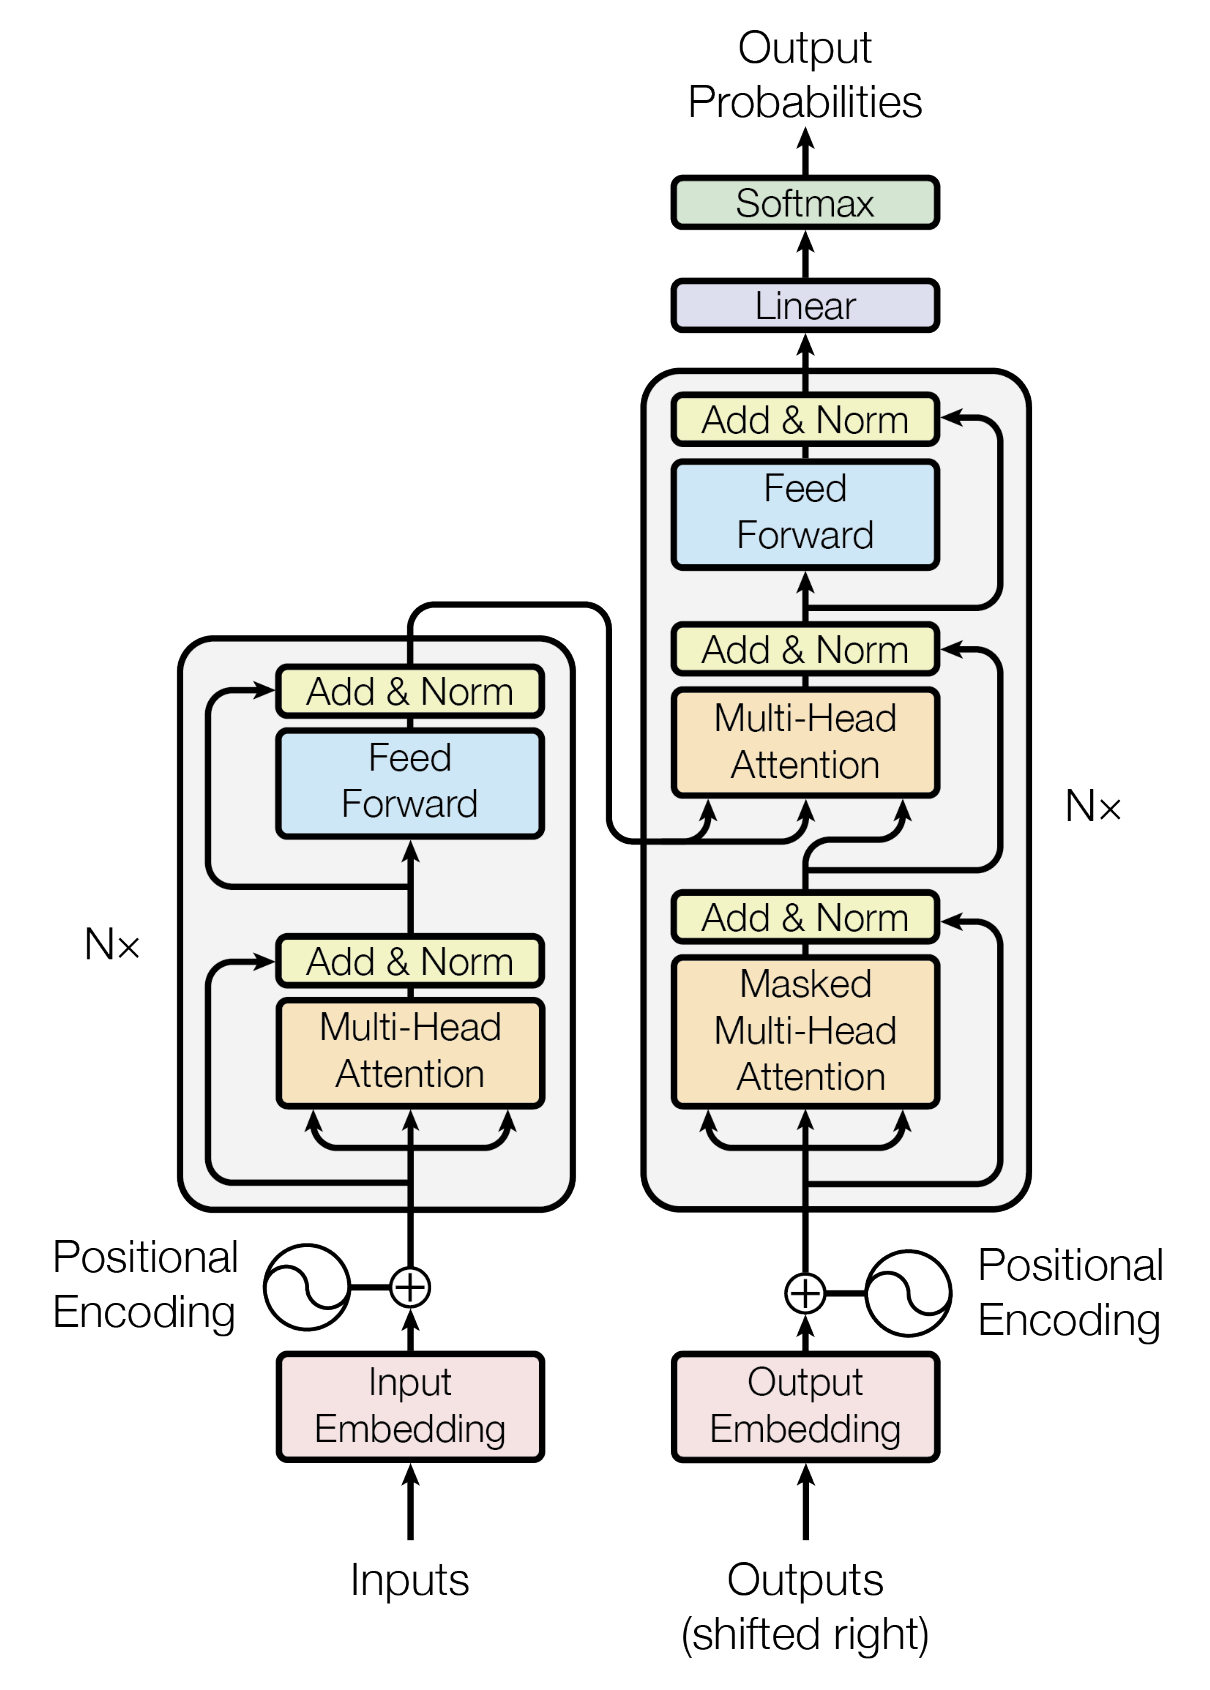
\includegraphics[width=4cm]{data/transformer.png}
            };
            \node[draw=red, thick, minimum width=1cm, minimum height=0.28cm] at (5.65, 4.98) {};
        \end{tikzpicture}
    \end{frame}
    \begin{frame}{Transformers: Demo}
        \centering
        \begin{tikzpicture}
            \node[] at (0, 0) {};
            \node[] at (10, 7) {};
            \only<1>{
                \node[] at (5, 3.5) {
                    {\scriptsize
                        \url{https://huggingface.co/docs/transformers/model_doc/llama2}
                    }
                };
            }
            \only<2>{
                \node[] at (5, 3.5) {
                    {\scriptsize
                        \url{http://localhost:8888/notebooks/notebooks/GPT\%20Embedding.ipynb}
                    }
                };
            }
        \end{tikzpicture}
    \end{frame}
    \begin{frame}{Transformers}
        Transformers: Revolutionized language modelling by combining feed forward neural networks with multihead attention and positional endcodings (and infinite data and compute)
            \begin{itemize}
                \item Main advantage: Outperforms everything else for almost all language modelling tasks
                \item Main disadvantage: Can either be used locally, which is fidgety and requires a good computer, or via an API, which is costly and gives others access to your data
            \end{itemize}
    \end{frame}
\end{document}
